\documentclass[12pt,a4paper,twoside]{report}
% -------------------------------------------------------------------- %
% Pacotes

\usepackage[utf8]{inputenc}
\usepackage[T1]{fontenc}
\usepackage[brazil]{babel}
\usepackage[fixlanguage]{babelbib}
\usepackage[pdftex]{graphicx}      % usamos arquivos pdf/png como figuras
\usepackage{setspace}              % espaçamento flexvel
\usepackage{indentfirst}           % indentação do primeiro parágrafo
\usepackage{makeidx}               % índice remissivo
\usepackage[nottoc]{tocbibind}     % acrescentamos a bibliografia/indice/conteudo no Table of Contents
\usepackage{courier}               % usa o Adobe Courier no lugar de Computer Modern Typewriter
\usepackage{type1cm}               % fontes realmente escaláveis
\usepackage{titletoc}
\usepackage{ucs}
\usepackage[font=small,format=plain,labelfont=bf,up,textfont=it,up]{caption}
\usepackage[usenames,svgnames,dvipsnames]{xcolor}
\usepackage[a4paper,top=2.54cm,bottom=2.0cm,left=2.0cm,right=2.54cm]{geometry} % margens
\usepackage{amsmath} 
\usepackage{float}

\usepackage[pdftex,plainpages=false,pdfpagelabels,pagebackref,colorlinks=true,citecolor=DarkGreen,
linkcolor=NavyBlue,urlcolor=DarkRed,filecolor=green,bookmarksopen=true]{hyperref} % links coloridos
\usepackage[all]{hypcap}                % soluciona o problema com o hyperref e capítulos
\usepackage[square,sort,nonamebreak,comma]{natbib}  % citação bibliográfica alpha
\fontsize{60}{62}\usefont{OT1}{cmr}{m}{n}{\selectfont}
\usepackage{upquote}                    % formata apóstrofes '
\usepackage{textcomp}

% Para formatar corretamente as URLs
\usepackage{url}
% -------------------------------------------------------------------- %
% Cabeçalhos similares ao TAOCP de Donald E. Knuth
\usepackage{fancyhdr}
\pagestyle{fancy}
\fancyhf{}
\renewcommand{\chaptermark}[1]{\markboth{\MakeUppercase{#1}}{}}
\renewcommand{\sectionmark}[1]{\markright{\MakeUppercase{#1}}{}}
\renewcommand{\headrulewidth}{0pt}

% -------------------------------------------------------------------- %
\graphicspath{{./imagens/}}        % caminho das figuras
\frenchspacing                     % arruma o espaço: id est (i.e.) e exempli gratia (e.g.)
\urlstyle{same}                    % URL com o mesmo estilo do texto e no mono-spaced
\makeindex                         % para o índice remissivo
\raggedbottom                      % para no permitir espaços extras no texto
\fontsize{60}{62}\usefont{OT1}{cmr}{m}{n}{\selectfont}
\cleardoublepage
\normalsize

% -------------------------------------------------------------------- %
% Cores para formatação de código
\usepackage{color}
\definecolor{vermelho}{rgb}{0.6,0,0} % para strings
\definecolor{verde}{rgb}{0.25,0.5,0.35} % para comentários
\definecolor{roxo}{rgb}{0.5,0,0.35} % para palavras-chaves
\definecolor{azul}{rgb}{0.25,0.35,0.75} % para strings
\definecolor{cinza-claro}{gray}{0.95}
% -------------------------------------------------------------------- %
% Opções de listagem usados para o código fonte
% Ref: http://en.wikibooks.org/wiki/LaTeX/Packages/Listings



\usepackage{listings}           % para formatar código-fonte (ex. em Java)


\lstset{ %
language=[Objective]Caml,  % seleciona a linguagem do código (aqui em lstlang0.sty
basicstyle=\footnotesize\ttfamily, % o tamanho da fonte usado no código
commentstyle=\color{verde}\bfseries,  % formatação de comentários
stringstyle=\color{azul},    % formatação de strings
upquote=true,
numbers=left,                   % onde colocar os números de linha
numberstyle=\tiny,  % o tamanho da fonte usada para a numeração das linhas
stepnumber=1,                   % o intervalo entre dois números de linhas. Se for 1, numera cada uma.
numbersep=5pt,                  % how far the line-numbers are from the code
showspaces=false,               % show spaces adding particular underscores
showstringspaces=false,         % underline spaces within strings
showtabs=false,                 % show tabs within strings adding particular underscores
keywordstyle=\color{roxo}\bfseries,
keywordstyle=[1]\color{roxo}\bfseries,
keywordstyle=[2]\color{verde}\bfseries,
%        keywordstyle=[3]\textbf,    %
%        keywordstyle=[4]\textbf,   \sqrt{\sqrt{}} %
frame=b,                   % adds a frame around the code
framerule=0.6pt,
tabsize=2,                      % sets default tabsize to 2 spaces
captionpos=t,                   % sets the caption-position to top
breaklines=true,                % sets automatic line breaking
breakatwhitespace=false,        % sets if automatic breaks should only happen at whitespace
escapeinside={\%*}{*)},         % if you want to add a comment within your code
backgroundcolor=\color[rgb]{1.0,1.0,1.0}, % choose the background color.
rulecolor=\color[rgb]{0.8,0.8,0.8},
extendedchars=true,
xleftmargin=10pt,
xrightmargin=10pt,
framexleftmargin=10pt,
framexrightmargin=10pt,
literate={â}{{\^{a}}}1  % para formatar corretamente os acentos do Português ao usar utf8
    {ê}{{\^{e}}}1
    {ô}{{\^{o}}}1  
    {Â}{{\^{A}}}1
    {Ê}{{\^{E}}}1
    {Ô}{{\^{O}}}1
    {á}{{\'{a}}}1
    {é}{{\'{e}}}1
    {í}{{\'{i}}}1
    {ó}{{\'{o}}}1
    {ú}{{\'{u}}}1
    {Á}{{\'{A}}}1
    {É}{{\'{E}}}1
    {Í}{{\'{I}}}1
    {Ó}{{\'{O}}}1
    {Ú}{{\'{U}}}1
    {à}{{\`{a}}}1
    {À}{{\`{A}}}1
    {ã}{{\~{a}}}1
    {õ}{{\~{o}}}1
    {Ã}{{\~{A}}}1
    {Õ}{{\~{O}}}1
    {ç}{{\c{c}}}1
    {Ç}{{\c{C}}}1
    {ü}{{\"u}}1
    {Ü}{{\"U}}1
}

\renewcommand{\lstlistingname}{Listagem}
\renewcommand{\lstlistlistingname}{Lista de Listagens}

% Definição de novos estilos
\lstdefinestyle{Bash}
    {language=bash,frame=single,numbers=none,basicstyle=\footnotesize\ttfamily,
     morekeywords={cp,mkdir,sudo,tar}}

% Definição de novos ambientes
\lstnewenvironment{terminal}
  {\lstset{style=Bash}}
  {}

\lstnewenvironment{ocaml}
  {\lstset{basicstyle=\scriptsize\ttfamily,
           frame=single,
           frameround=tttt,
           framerule=2pt,
           numbers=none,
           rulecolor=\color{Salmon}}}
  {}

\lstnewenvironment{xml}
   {\lstset{language=XML,frame=single,numbers=none}}
   {}

\lstnewenvironment{interprete}
  {\lstset{frame=single,
            frameround=tttt,
            numbers=none,
            basicstyle=\ttfamily,
            framerule=2pt,
            rulecolor=\color{CadetBlue}}}
  {}
% Formata o caption da listagem
% \DeclareCaptionFont{blue}{\color{blue}} 

% \captionsetup[lstlisting]{singlelinecheck=false, labelfont={blue}, textfont={blue}}
\usepackage{caption}
\DeclareCaptionFont{white}{\color{white}}
\DeclareCaptionFormat{listing}{\colorbox[cmyk]{0.43, 0.35, 0.35,0.01}{\parbox{\textwidth}{\hspace{15pt}#1#2#3}}}
\captionsetup[lstlisting]{format=listing,labelfont=white,textfont=white, singlelinecheck=false, margin=0pt, font={bf,footnotesize}}

\newcommand{\ListingsPath}{./codigos}
% Inclui o nome do arquivo como Caption 
\newcommand{\filelisting}[2][]{%
    \lstinputlisting[caption={\texttt{\detokenize{#2}}},#1]{\ListingsPath/#2}%
}

% ---------------------------------------------------------------------------- %

% ---------------------------------------------------------------------------- %

\title{Análise de Algoritmos - Algoritmos Diversos}
\date{}
\author{Gustavo de Souza Silva \\ Guilherme de Souza Silva \\ Arthur Xavier \\ Schumaiquer Souto \\
\vspace{1cm} \\
Faculdade de Computação \\
Universidade Federal de Uberlândia
}
\date{\today}

%\includeonly{cap-clojure,magical,short}
\begin{document}
  \maketitle
% -------------------------------------------------------------------- %
% Listas de figuras, tabelas e códigos criadas automaticamente
\listoffigures            
\listoftables            
\lstlistoflistings
% -------------------------------------------------------------------- %

% -------------------------------------------------------------------- %
% Sumário
\tableofcontents    

% Capítulos do trabalho

% cabeçalho para as páginas de todos os capítulos
\fancyhead[RE,LO]{\thesection}

%\singlespacing              % espaçamento simples
\setlength{\parskip}{0.15in} % espaçamento entre paragráfos

\chapter{Introdução}
Este relatório tem como objetivo fazer a análise de diversos algoritmos já conhecidos de Busca, Gulosos, dinâmicos de de estatística de ordem. O intuito deste trabalho é comprovar que as provas matemáticas realmente acontecem em um ambiente real de execução.

\section{Codificação}
Arquivo dos gulosos e Programação Dinâmica
\lstinputlisting[label={arq:final.c}, language=C, caption={Arquivo dos gulosos e Programação Dinâmica}]{../final.c}

Arquivos com algoritmos de estatística de ordem
\lstinputlisting[label={arq:RandomizedSelect.c}, language=C, caption={Estatística de Ordem}]{../RandomizedSelect.c}

Arquivo contendo o algoritmo de huffman
\lstinputlisting[label={arq:huffman.c}, language=C, caption={Arquivo de Huffman}]{../huffman.c}

O arquivo vetor.c mantém todas as funções a respeito do vetor, como geração, preenchimento, etc.
\lstinputlisting[label={arq:grafo.c}, language=C, caption={Arquivo referente ao grafo}]{../grafo.c}

Este arquivo serve para gerar os vetores e salva-los em arquivos.
\lstinputlisting[label={arq:gera_grafo.c}, language=C, caption={Geração dos grafos}]{../gera_grafo.c}

Este arquivo contém os algoritmos de ordenação pedidos.
\lstinputlisting[label={arq:opgrafo.c}, language=C, caption={Métodos de busca}]{../opgrafo.c}

O arquivo ensaios.c serve para automatizar e calcular os tempos de cada método de ordenação.
\lstinputlisting[label={arq:ensaiosgrafo.c}, language=C, caption={Automatização dos experimentos}]{../ensaiosgrafo.c}

\subsection{Comandos}
Os seguintes passos devem ser seguidos para criação dos grafos que serão utilizados no experimento:\\
1 - Compilar o arquivo Grafo.c;
\begin{terminal}
    > gcc -O3 -c grafo.c
    > gcc -O3 -c opgrafo.c
\end{terminal}
2 - Compilar o programa que gera os grafos e os coloca no diretório determinado;
\begin{terminal}
    > gcc -O3 grafi.o gera_grafo.c -o gera_grafo.exe
\end{terminal}
3 - Para usá-lo digite
\begin{terminal}
    > ./gera_grafos.exe
\end{terminal}

Os passos a seguir são para execução do experimento\\
1 - Verifique a existência do diretório contendo os grafos, e então digite o seguinte comando:
\begin{terminal}
    > gcc -O3 -c opgrafo.c
\end{terminal}
2 - Agora é necessário compilar o arquivo de ensaio e tudo que será utilizado
\begin{terminal}
    > gcc -O3 grafo.o opgrafo.o ensaiosgrafo.c -o ensaiosgrafo.exe -lm
\end{terminal}
3 - Para executar digite:
\begin{terminal}
    > ./ensaiosgrafo.exe
\end{terminal}

\section{Máquina de teste}
Todos os testes foram realizados na mesma máquina com as seguintes configurações, e usando apenas um núcleo:\\
AMD FX-8350 4.0GHZ\\
16GB Memória DDR3-1600\\
HDD 2TB 7200RPM\\
Placa de video Nvidia GTX1050Ti\\
Sistema Operacional: Ubuntu 16.04\\

\chapter{Grafo}

A teoria dos grafos é um ramo da matemática que estuda as relações entre os objetos de um determinado conjunto. Para tal são empregadas estruturas chamadas de grafos, G(V,E), onde V é um conjunto não vazio de objetos denominados vértices e E é um subconjunto de pares não ordenados de V, chamados arestas. Neste trabalho, foi-se definido como grafo esparso um grafo que tem apenas uma aresta entre cada par de vértice (1~2,2~3,3~4,...n-1~n) e um granfo denso foi definido como um grafo completo, ou seja, cada vértice tem aresta com todos os outros vértices.

\section{Busca Largura}

É um algoritmo de busca em grafos utilizado para realizar uma busca ou travessia num grafo e estrutura de dados do tipo árvore. Você começa pelo vértice raiz e explora todos os vértices vizinhos. Então, para cada um desses vértices mais próximos, exploramos os seus vértices vizinhos inexplorados e assim por diante, até que ele encontre o alvo da busca.

\section{Busca Largura - Grafo Esparso}
\begin{table}[H]
\centering
\caption{Busca Largura com grafo Esparso}
\begin{tabular}{|l|l|}
\hline
\multicolumn{1}{|c|}{\textbf{Número de Elementos}} & \multicolumn{1}{c|}{\textbf{Tempo de execução em nanosegundos}} \\ \hline
128 & 7943 \\ \hline
256 & 7472 \\ \hline
512 & 15414 \\ \hline
1024 & 32102 \\ \hline
\end{tabular}
\end{table}

\subsection{Gráfico Busca Largura - Grafo Esparso}
\begin{figure}[H]
    \centering
    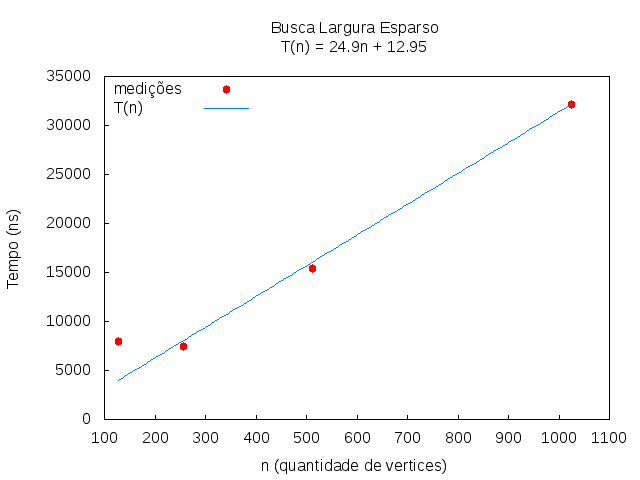
\includegraphics[width=0.7\linewidth]{graficos/BuscaLargura/Esparso/Esparso.png}
  \caption{Busca Largura - Grafo Esparso}
\end{figure}

\section{Busca Largura - Grafo Denso}

\begin{table}[H]
\centering
\caption{Busca em Largura Grafo Denso}
\label{my-label}
\begin{tabular}{|l|l|}
\hline
\multicolumn{1}{|c|}{\textbf{Número de Elementos}} & \multicolumn{1}{c|}{\textbf{Tempo de execução em nanosegundos}} \\ \hline
128 & 67546 \\ \hline
256 & 318565 \\ \hline
512 & 1216634 \\ \hline
1024 & 4527417 \\ \hline
\end{tabular}
\end{table}

\subsection{Busca em Largura - Grafo Denso}
\begin{figure}[H]
    \centering
    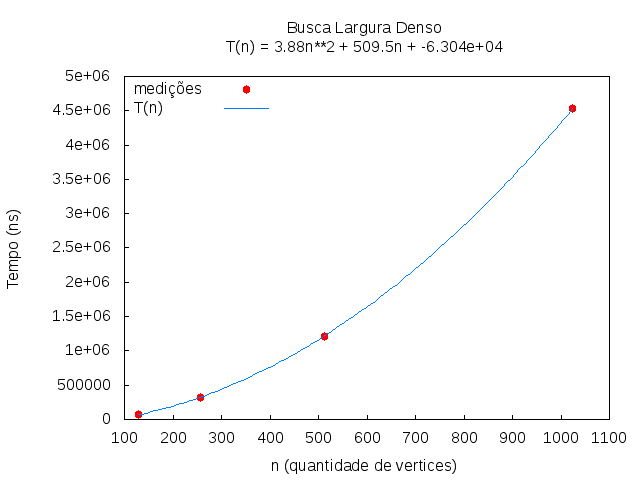
\includegraphics[width=0.7\linewidth]{graficos/BuscaLargura/Denso/Denso.png}
  \caption{Busca em Largura - Grafo Denso}
\end{figure}

\section{Busca Profundidade}
É um algoritmo usado para realizar uma busca ou travessia numa árvore, estrutura de árvore ou grafo. O algoritmo começa num nó raiz (selecionando algum nó como sendo o raiz, no caso de um grafo) e explora tanto quanto possível cada um dos seus ramos, antes de retroceder(backtracking).

\section{Busca Profundidade - Grafo Esparso}
\begin{table}[H]
\centering
\caption{Busca Profundidade com Grafo Esparso}
\label{my-label}
\begin{tabular}{|l|l|}
\hline
\multicolumn{1}{|c|}{\textbf{Número de Elementos}} & \multicolumn{1}{c|}{\textbf{Tempo de execução em nanosegundos}} \\ \hline
128 & 6619 \\ \hline
256 & 7975 \\ \hline
512 & 21265 \\ \hline
1024 & 36223 \\ \hline
\end{tabular}
\end{table}

\subsection{Busca Profundidade - Grafo Esparso}
\begin{figure}[H]
    \centering
    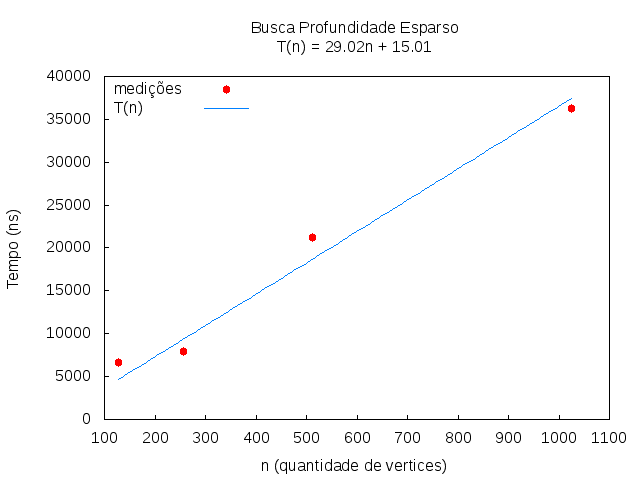
\includegraphics[width=0.7\linewidth]{graficos/BuscaProfundidade/Esparso/Esparso.png}
  \caption{Busca Profundidade - Grafo Esparso}
\end{figure}

\section{Busca Profundidade - Grafo Denso}
\begin{table}[H]
\centering
\caption{Busca Profundidade em um Grafo Denso}
\label{my-label}
\begin{tabular}{|l|l|}
\hline
\multicolumn{1}{|c|}{\textbf{Número de Elementos}} & \multicolumn{1}{c|}{\textbf{Tempo de execução em nanosegundos}} \\ \hline
128 & 72161 \\ \hline
256 & 330916 \\ \hline
512 & 1380078 \\ \hline
1024 & 4735134 \\ \hline
\end{tabular}
\end{table}

\subsection{Busca Profundidade - Grafo Denso}
\begin{figure}[H]
    \centering
    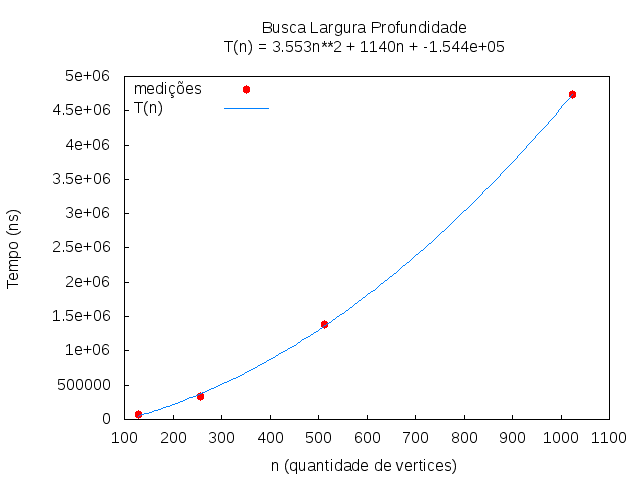
\includegraphics[width=0.7\linewidth]{graficos/BuscaProfundidade/Denso/Denso.png}
  \caption{Busca Profundidade - Grafo Denso}
\end{figure}

\section{Ordenação Topologica}

 É uma ordem linear de seus nós em que cada nó vem antes de todos nós para os quais este tenha arestas de saída. Cada DAG tem uma ou mais ordenações topológicas.

\section{Ordenação Topologica - Grafo Esparso}
\begin{table}[H]
\centering
\caption{Ordenação Topologica com Grafo Esparso}
\label{my-label}
\begin{tabular}{|l|l|}
\hline
\multicolumn{1}{|c|}{\textbf{Número de Elementos}} & \multicolumn{1}{c|}{\textbf{Tempo de execução em nanosegundos}} \\ \hline
128 & 13549 \\ \hline
256 & 15347 \\ \hline
512 & 30745 \\ \hline
1024 & 57293 \\ \hline
\end{tabular}
\end{table}

\subsection{Ordenação Topologica - Grafo Esparso}
\begin{figure}[H]
    \centering
    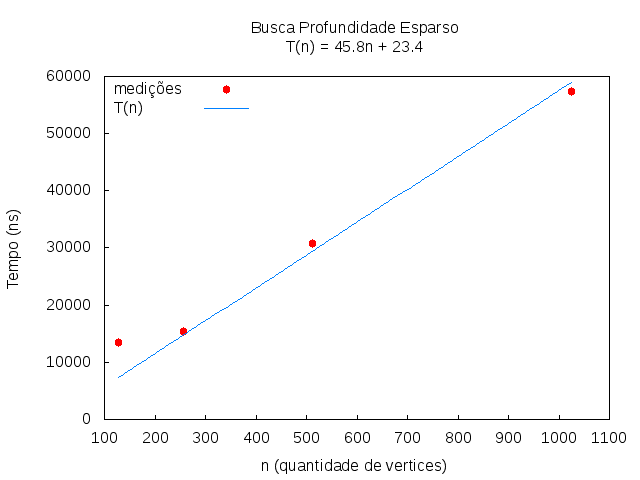
\includegraphics[width=0.7\linewidth]{graficos/OrdenaTopologico/Esparso/Esparso.png}
  \caption{Ordenação Topologica - Grafo Esparso}
\end{figure}

\section{Ordenação Topologica - Grafo Denso}
\begin{table}[H]
\centering
\caption{Ordenação Topologica com Grafo Denso}
\label{my-label}
\begin{tabular}{|l|l|}
\hline
\multicolumn{1}{|c|}{\textbf{Número de Elementos}} & \multicolumn{1}{c|}{\textbf{Tempo de execução em nanosegundos}} \\ \hline
128 & 93864 \\ \hline
256 & 349061 \\ \hline
512 & 1344655 \\ \hline
1024 & 4865168 \\ \hline
\end{tabular}
\end{table}

\subsection{Ordenação Topologica - Grafo Denso}
\begin{figure}[H]
    \centering
    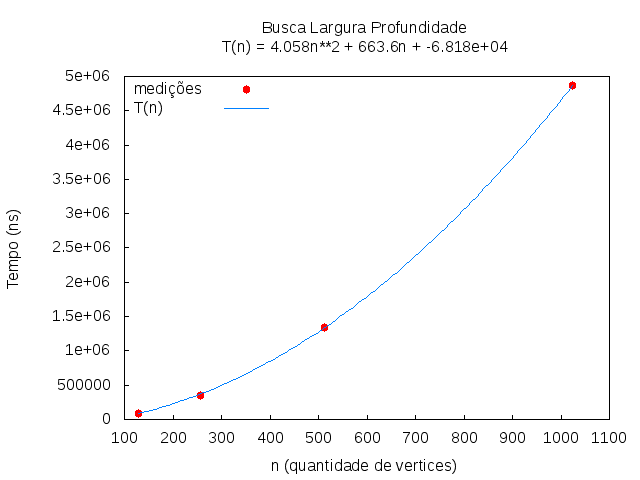
\includegraphics[width=0.7\linewidth]{graficos/OrdenaTopologico/Denso/Denso.png}
  \caption{Ordenação Topologica - Grafo Denso}
\end{figure}

\chapter{Guloso}

Algoritmo guloso ou míope é técnica de projeto de algoritmos que tenta resolver o problema fazendo a escolha localmente ótima em cada fase com a esperança de encontrar um ótimo global.

\section{Huffman}

A codificação de Huffman é um método de compressão que usa as probabilidades de ocorrência dos símbolos no conjunto de dados a ser comprimido para determinar códigos de tamanho variável para cada símbolo.

\subsection{Vetor aleatorio}
Tabela gerada utilizando Huffman com vetor de string aleatorias com frequencias em tempo O(nlogn) de tamanho n, sendo n = $(2^k)$, de k = 4..14 e inseridos aleatóriamente.
\begin{table}[H]
\centering
\caption{Huffman com vetor aleatório}
\label{my-label}
\begin{tabular}{|l|l|}
\hline
\multicolumn{1}{|c|}{\textbf{Número de Elementos}} & \multicolumn{1}{c|}{\textbf{Tempo de execução em nanosegundos}} \\ \hline
16 & 4599 \\ \hline
32 & 8150 \\ \hline
64 & 22736 \\ \hline
128 & 42886 \\ \hline
256 & 95255 \\ \hline
512 & 170503 \\ \hline
1024 & 438873 \\ \hline
2048 & 1031620 \\ \hline
4096 & 2592036 \\ \hline
8192 & 5381493 \\ \hline
16384 & 10506005 \\ \hline

\end{tabular}
\end{table}

\begin{figure}[H]
    \centering
    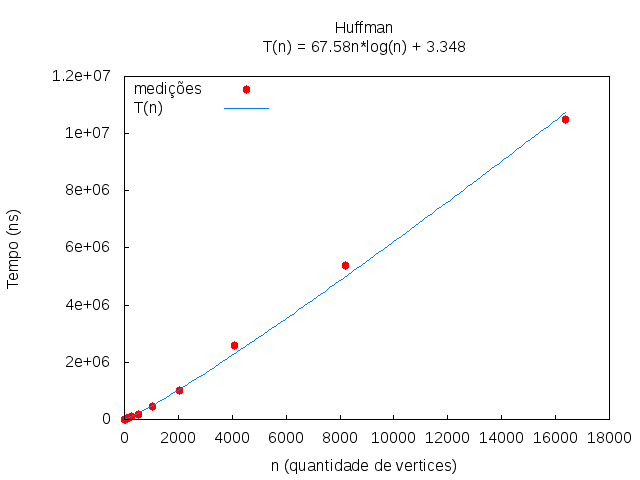
\includegraphics[width=0.7\linewidth]{graficos/Huffman/Huffman.png}
  \caption{Huffman - Vetor Aleatório}
\end{figure}

\section{Seleção de Atividade Interativo}

É um problema onde dado um conjunto S de atividades, encontrar o maior subconjunto de S com
atividades mutuamente compatíveis.

\subsection{Vetor crescente}
Tabela gerada utilizando Seleção de Atividade Interativo com vetor de tamanho n, sendo n = $(2^k)$, de k = 4..14 e inseridos crescente.
\begin{table}[H]
\centering
\caption{Seleção de Atividade Interativo com vetor crescente}
\label{my-label}
\begin{tabular}{|l|l|}
\hline
\multicolumn{1}{|c|}{\textbf{Número de Elementos}} & \multicolumn{1}{c|}{\textbf{Tempo de execução em nanosegundos}} \\ \hline
16 & 615 \\ \hline
32 & 680 \\ \hline
64 & 769 \\ \hline
128 & 802 \\ \hline
256 & 764 \\ \hline
512 & 836 \\ \hline
1024 & 1058 \\ \hline
2048 & 1294 \\ \hline
4096 & 1685 \\ \hline
8192 & 2594 \\ \hline
16384 & 4578 \\ \hline

\end{tabular}
\end{table}

\begin{figure}[H]
    \centering
    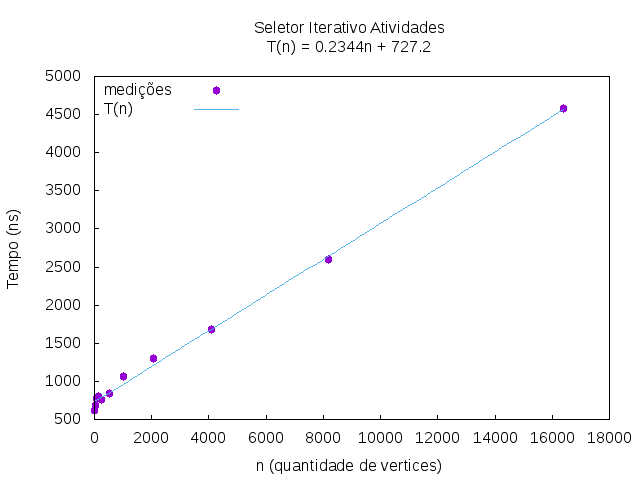
\includegraphics[width=0.7\linewidth]{graficos/SeletorIterativoAtividades/SeletorIterativoAtividades.png}
  \caption{Seleção de Atividade Interativo - Vetor crescente}
\end{figure}

\section{Seletor Recursivo de Atividade}

É um problema onde dado um conjunto S de atividades, encontrar o maior subconjunto de S com
atividades mutuamente compatíveis.

\subsection{Vetor Aleatório}
Tabela gerada utilizando Seleção de Atividade Interativo com vetor de tamanho n, sendo n = $(2^k)$, de k = 4..14 e inseridos aleatório.
\begin{table}[H]
\centering
\caption{Seleciona Recursivo de Atividade de Atividade de Atividade de Atividade de Atividade de Atividade de Atividade de Atividade de Atividade de Atividade de Atividade com vetor aleatório}
\label{my-label}
\begin{tabular}{|l|l|}
\hline
\multicolumn{1}{|c|}{\textbf{Número de Elementos}} & \multicolumn{1}{c|}{\textbf{Tempo de execução em nanosegundos}} \\ \hline
16 & 848 \\ \hline
32 & 859 \\ \hline
64 & 1226 \\ \hline
128 & 2086 \\ \hline
256 & 3352 \\ \hline
512 & 4632 \\ \hline
1024 & 10637 \\ \hline
2048 & 24606 \\ \hline
4096 & 40615 \\ \hline
8192 & 88004 \\ \hline
16384 & 135617 \\ \hline

\end{tabular}
\end{table}

\begin{figure}[H]
    \centering
    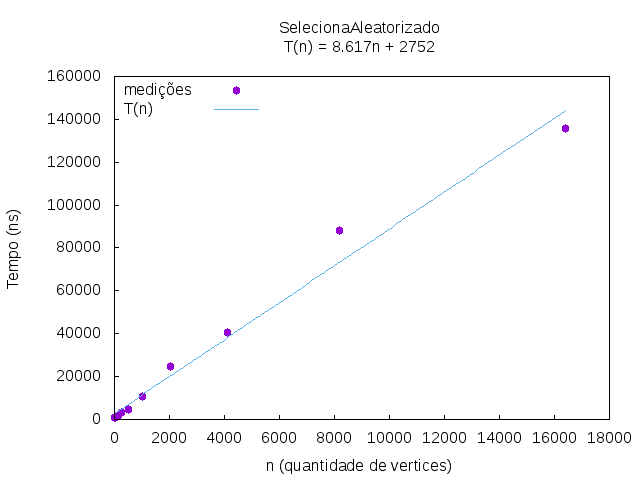
\includegraphics[width=0.7\linewidth]{graficos/SeletorRecursivoAtividades/Aleatorio/SelecionaAleatorizado.png}
  \caption{Seleciona Recursivo de Atividade - Vetor Aleatório}
\end{figure}


\subsection{Vetor Crescente}
Tabela gerada utilizando Seleciona Recursivo de Atividade com vetores de tamanho n, sendo n = $(2^k)$, de k = 4..14 e inseridos Crescente.
\begin{table}[H]
\centering
\caption{Seleciona Recursivo de Atividade com vetor crescente}
\label{my-label}
\begin{tabular}{|l|l|}
\hline
\multicolumn{1}{|c|}{\textbf{Número de Elementos}} & \multicolumn{1}{c|}{\textbf{Tempo de execução em nanosegundos}} \\ \hline
16 & 563 \\ \hline
32 & 677 \\ \hline
64 & 1184 \\ \hline
128 & 2093 \\ \hline
256 & 3518 \\ \hline
512 & 6070 \\ \hline
1024 & 9960 \\ \hline
2048 & 24854 \\ \hline
4096 & 39433 \\ \hline
8192 & 79908 \\ \hline
16384 & 245208 \\ \hline

\end{tabular}
\end{table}

\begin{figure}[H]
    \centering
    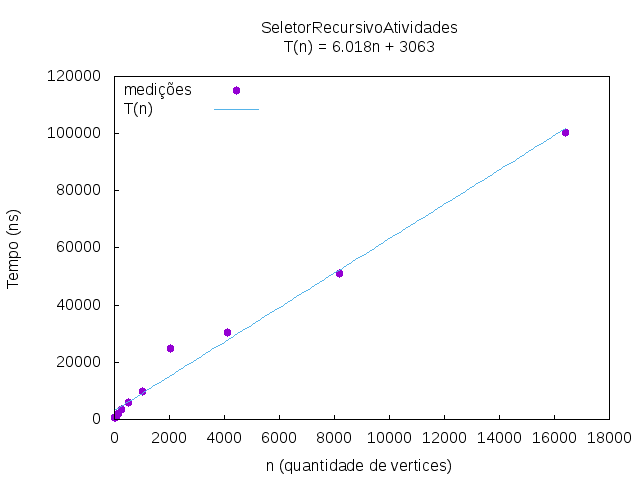
\includegraphics[width=0.7\linewidth]{graficos/SeletorRecursivoAtividades/Crescente/SelecionaAleatorizado.png}
  \caption{Seleciona Recursivo de Atividade - Vetor crescente}
\end{figure}


\subsection{Vetor Crescente P10}
Tabela gerada utilizando Seleciona Recursivo de Atividade  com vetores de tamanho n, sendo n = $(2^k)$, de k = 4..14 e inseridos Crescente P10.
\begin{table}[H]
\centering
\caption{Seleciona Recursivo de Atividade com vetor crescente P10}
\label{my-label}
\begin{tabular}{|l|l|}
\hline
\multicolumn{1}{|c|}{\textbf{Número de Elementos}} & \multicolumn{1}{c|}{\textbf{Tempo de execução em nanosegundos}} \\ \hline
16 & 672 \\ \hline
32 & 843 \\ \hline
64 & 1091 \\ \hline
128 & 2310 \\ \hline
256 & 3383 \\ \hline
512 & 6038 \\ \hline
1024 & 19242 \\ \hline
2048 & 34439 \\ \hline
4096 & 46022 \\ \hline
8192 & 95304 \\ \hline
16384 & 176781 \\ \hline

\end{tabular}
\end{table}

\begin{figure}[H]
    \centering
    \includegraphics[width=0.7\linewidth]{graficos/SeletorRecursivoAtividades/Crescente P10/SelecionaAleatorizado.png}
  \caption{Seleciona Recursivo de Atividade - Vetor crescente P10}
\end{figure}



\subsection{Vetor Crescente P20}
Tabela gerada utilizando Seleciona Recursivo de Atividade com vetores de tamanho n, sendo n = $(2^k)$, de k = 4..14 e inseridos Crescente P20.
\begin{table}[H]
\centering
\caption{Seleciona Recursivo de Atividade com vetor crescente P20}
\label{my-label}
\begin{tabular}{|l|l|}
\hline
\multicolumn{1}{|c|}{\textbf{Número de Elementos}} & \multicolumn{1}{c|}{\textbf{Tempo de execução em nanosegundos}} \\ \hline
16 & 613 \\ \hline
32 & 780 \\ \hline
64 & 1259 \\ \hline
128 & 1836 \\ \hline
256 & 2640 \\ \hline
512 & 9910 \\ \hline
1024 & 11045 \\ \hline
2048 & 19416 \\ \hline
4096 & 46564 \\ \hline
8192 & 86621 \\ \hline
16384 & 198014 \\ \hline

\end{tabular}
\end{table}

\begin{figure}[H]
    \centering
    \includegraphics[width=0.7\linewidth]{graficos/SeletorRecursivoAtividades/Crescente P20/SelecionaAleatorizado.png}
  \caption{Seleciona Recursivo de Atividade - Vetor crescente P20}
\end{figure}



\subsection{Vetor Crescente P30}
Tabela gerada utilizando Seleciona Recursivo de Atividade com vetores de tamanho n, sendo n = $(2^k)$, de k = 4..14 e inseridos Crescente P30.
\begin{table}[H]
\centering
\caption{Seleciona Recursivo de Atividade com vetor crescente P30}
\label{my-label}
\begin{tabular}{|l|l|}
\hline
\multicolumn{1}{|c|}{\textbf{Número de Elementos}} & \multicolumn{1}{c|}{\textbf{Tempo de execução em nanosegundos}} \\ \hline
16 & 651 \\ \hline
32 & 698 \\ \hline
64 & 1008 \\ \hline
128 & 2052 \\ \hline
256 & 3051 \\ \hline
512 & 6192 \\ \hline
1024 & 10526 \\ \hline
2048 & 17150 \\ \hline
4096 & 45699 \\ \hline
8192 & 76166 \\ \hline
16384 & 155111 \\ \hline
\end{tabular}
\end{table}

\begin{figure}[H]
    \centering
    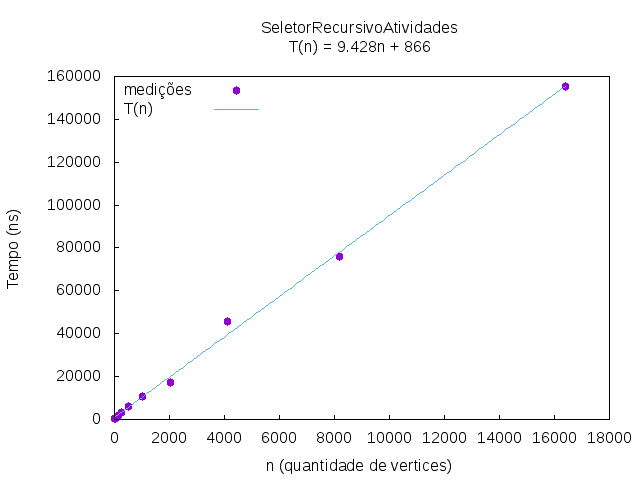
\includegraphics[width=0.7\linewidth]{graficos/SeletorRecursivoAtividades/Crescente P30/SelecionaAleatorizado.png}
  \caption{Seleciona Recursivo de Atividade - Vetor crescente P30}
\end{figure}


\subsection{Vetor Crescente P40}
Tabela gerada utilizando Seleciona Recursivo de Atividade com vetores de tamanho n, sendo n = $(2^k)$, de k = 4..14 e inseridos Crescente P40.
\begin{table}[H]
\centering
\caption{Seleciona Recursivo de Atividade com vetor crescente P40}
\label{my-label}
\begin{tabular}{|l|l|}
\hline
\multicolumn{1}{|c|}{\textbf{Número de Elementos}} & \multicolumn{1}{c|}{\textbf{Tempo de execução em nanosegundos}} \\ \hline
16 & 743 \\ \hline
32 & 666 \\ \hline
64 & 989 \\ \hline
128 & 1508 \\ \hline
256 & 2883 \\ \hline
512 & 5360 \\ \hline
1024 & 11656 \\ \hline
2048 & 20539 \\ \hline
4096 & 41529 \\ \hline
8192 & 100858 \\ \hline
16384 & 222297 \\ \hline

\end{tabular}
\end{table}

\begin{figure}[H]
    \centering
    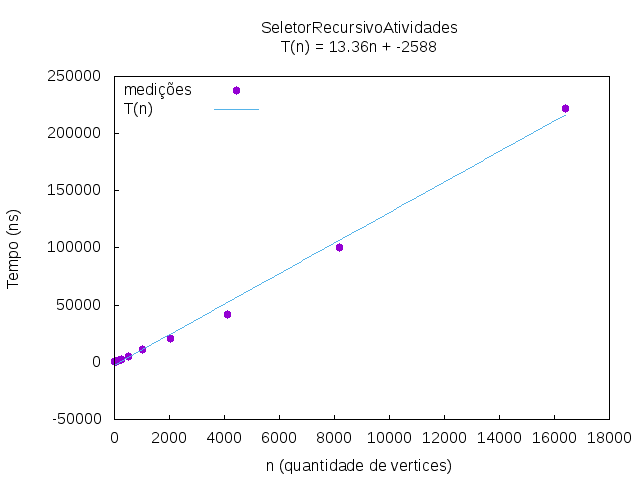
\includegraphics[width=0.7\linewidth]{graficos/SeletorRecursivoAtividades/Crescente P40/SelecionaAleatorizado.png}
  \caption{Seleciona Recursivo de Atividade - Vetor crescente P40}
\end{figure}




\subsection{Vetor Crescente P50}
Tabela gerada utilizando Seleciona Recursivo de Atividade com vetores de tamanho n, sendo n = $(2^k)$, de k = 4..14 e inseridos Crescente P50.
\begin{table}[H]
\centering
\caption{Seleciona Recursivo de Atividade com vetor crescente P50}
\label{my-label}
\begin{tabular}{|l|l|}
\hline
\multicolumn{1}{|c|}{\textbf{Número de Elementos}} & \multicolumn{1}{c|}{\textbf{Tempo de execução em nanosegundos}} \\ \hline
16 & 620 \\ \hline
32 & 827 \\ \hline
64 & 1258 \\ \hline
128 & 1600 \\ \hline
256 & 3615 \\ \hline
512 & 4546 \\ \hline
1024 & 10992 \\ \hline
2048 & 24860 \\ \hline
4096 & 60197 \\ \hline
8192 & 98321 \\ \hline
16384 & 249566 \\ \hline

\end{tabular}
\end{table}

\begin{figure}[H]
    \centering
    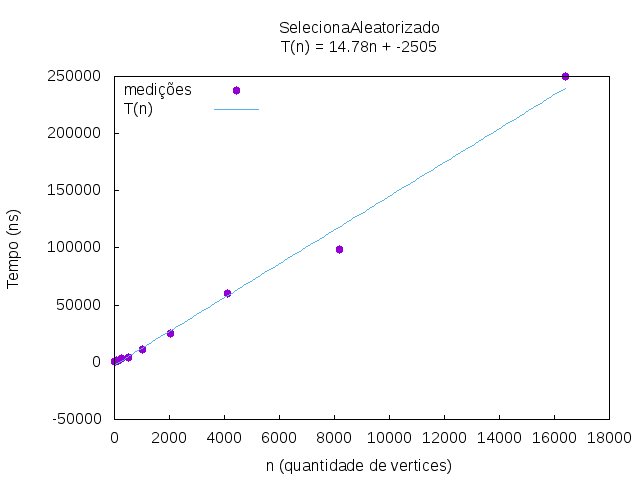
\includegraphics[width=0.7\linewidth]{graficos/SeletorRecursivoAtividades/Crescente P50/SelecionaAleatorizado.png}
  \caption{Seleciona Recursivo de Atividade - Vetor crescente P50}
\end{figure}


\subsection{Vetor Decrescente}
Tabela gerada utilizando Seleciona Recursivo de Atividade com vetores de tamanho n, sendo n = $(2^k)$, de k = 4..14 e inseridos Decrescente.
\begin{table}[H]
\centering
\caption{Seleciona Recursivo de Atividade com vetor decrescente}
\label{my-label}
\begin{tabular}{|l|l|}
\hline
\multicolumn{1}{|c|}{\textbf{Número de Elementos}} & \multicolumn{1}{c|}{\textbf{Tempo de execução em nanosegundos}} \\ \hline
16 & 822 \\ \hline
32 & 1130 \\ \hline
64 & 1610 \\ \hline
128 & 2075 \\ \hline
256 & 2774 \\ \hline
512 & 6371 \\ \hline
1024 & 12455 \\ \hline
2048 & 20537 \\ \hline
4096 & 39481 \\ \hline
8192 & 90849 \\ \hline
16384 & 216330 \\ \hline

\end{tabular}
\end{table}

\begin{figure}[H]
    \centering
    \includegraphics[width=0.7\linewidth]{graficos/SeletorRecursivoAtividades/Decrescente/SelecionaAleatorizado.png}
  \caption{Seleciona Recursivo de Atividade- Vetor decrescente}
\end{figure}




\subsection{Vetor Decrescente P10}
Tabela gerada utilizando Seleciona Recursivo de Atividade com vetores de tamanho n, sendo n = $(2^k)$, de k = 4..14 e inseridos Decrescente P10.
\begin{table}[H]
\centering
\caption{Seleciona Recursivo de Atividade com vetor decrescente P10}
\label{my-label}
\begin{tabular}{|l|l|}
\hline
\multicolumn{1}{|c|}{\textbf{Número de Elementos}} & \multicolumn{1}{c|}{\textbf{Tempo de execução em nanosegundos}} \\ \hline
16 & 692 \\ \hline
32 & 875 \\ \hline
64 & 968 \\ \hline
128 & 1772 \\ \hline
256 & 2865 \\ \hline
512 & 6142 \\ \hline
1024 & 10526 \\ \hline
2048 & 25677 \\ \hline
4096 & 46430 \\ \hline
8192 & 46738 \\ \hline
16384 & 177393 \\ \hline

\end{tabular}
\end{table}

\begin{figure}[H]
    \centering
    \includegraphics[width=0.7\linewidth]{graficos/SeletorRecursivoAtividades/Decrescente P10/SelecionaAleatorizado.png}
  \caption{Seleciona Recursivo de Atividade - Vetor decrescente P10}
\end{figure}



\subsection{Vetor Decrescente P20}
Tabela gerada utilizando Seleciona Recursivo de Atividade com vetores de tamanho n, sendo n = $(2^k)$, de k = 4..14 e inseridos Decrescente P20.
\begin{table}[H]
\centering
\caption{Seleciona Recursivo de Atividade com vetor decrescente P20}
\label{my-label}
\begin{tabular}{|l|l|}
\hline
\multicolumn{1}{|c|}{\textbf{Número de Elementos}} & \multicolumn{1}{c|}{\textbf{Tempo de execução em nanosegundos}} \\ \hline
16 & 963 \\ \hline
32 & 1130 \\ \hline
64 & 1209 \\ \hline
128 & 1862 \\ \hline
256 & 2040 \\ \hline
512 & 6190 \\ \hline
1024 & 14474 \\ \hline
2048 & 28032 \\ \hline
4096 & 58891 \\ \hline
8192 & 85015 \\ \hline
16384 & 191226 \\ \hline
\end{tabular}
\end{table}

\begin{figure}[H]
    \centering
    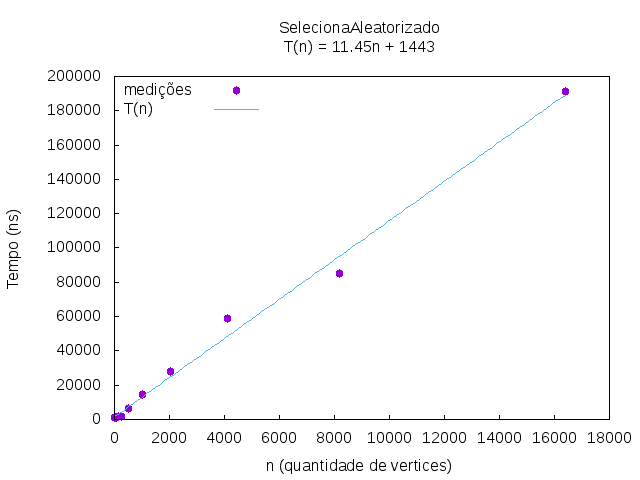
\includegraphics[width=0.7\linewidth]{graficos/SeletorRecursivoAtividades/Decrescente P20/SelecionaAleatorizado.png}
  \caption{Seleciona Recursivo de Atividade - Vetor decrescente P20}
\end{figure}



\subsection{Vetor Decrescente P30}
Tabela gerada utilizando Seleciona Recursivo de Atividade com vetores de tamanho n, sendo n = $(2^k)$, de k = 4..14 e inseridos Decrescente P30.
\begin{table}[H]
\centering
\caption{Seleciona Recursivo de Atividade com vetor decrescente P30}
\label{my-label}
\begin{tabular}{|l|l|}
\hline
\multicolumn{1}{|c|}{\textbf{Número de Elementos}} & \multicolumn{1}{c|}{\textbf{Tempo de execução em nanosegundos}} \\ \hline
16 & 691 \\ \hline
32 & 791 \\ \hline
64 & 1031 \\ \hline
128 & 1907 \\ \hline
256 & 3053 \\ \hline
512 & 9593 \\ \hline
1024 & 8715 \\ \hline
2048 & 11899 \\ \hline
4096 & 46642 \\ \hline
8192 & 64121 \\ \hline
16384 & 139003 \\ \hline

\end{tabular}
\end{table}

\begin{figure}[H]
    \centering
    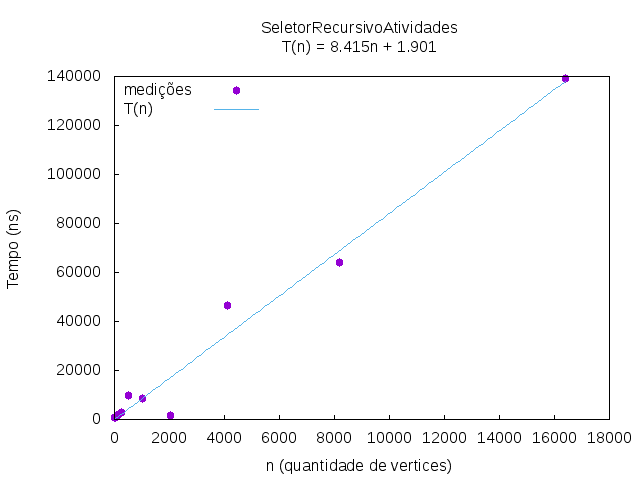
\includegraphics[width=0.7\linewidth]{graficos/SeletorRecursivoAtividades/Decrescente P30/SelecionaAleatorizado.png}
  \caption{Seleciona Recursivo de Atividade - Vetor decrescente P30}
\end{figure}




\subsection{Vetor Decrescente P40}
Tabela gerada utilizando Seleciona Recursivo de Atividade com vetores de tamanho n, sendo n = $(2^k)$, de k = 4..14 e inseridos Decrescente P40.
\begin{table}[H]
\centering
\caption{Seleciona Recursivo de Atividade com vetor decrescente P40}
\label{my-label}
\begin{tabular}{|l|l|}
\hline
\multicolumn{1}{|c|}{\textbf{Número de Elementos}} & \multicolumn{1}{c|}{\textbf{Tempo de execução em nanosegundos}} \\ \hline
16 & 818 \\ \hline
32 & 712 \\ \hline
64 & 1058 \\ \hline
128 & 1643 \\ \hline
256 & 2060 \\ \hline
512 & 4179 \\ \hline
1024 & 13014 \\ \hline
2048 & 22027 \\ \hline
4096 & 62149 \\ \hline
8192 & 101864 \\ \hline
16384 & 151244 \\ \hline

\end{tabular}
\end{table}

\begin{figure}[H]
    \centering
    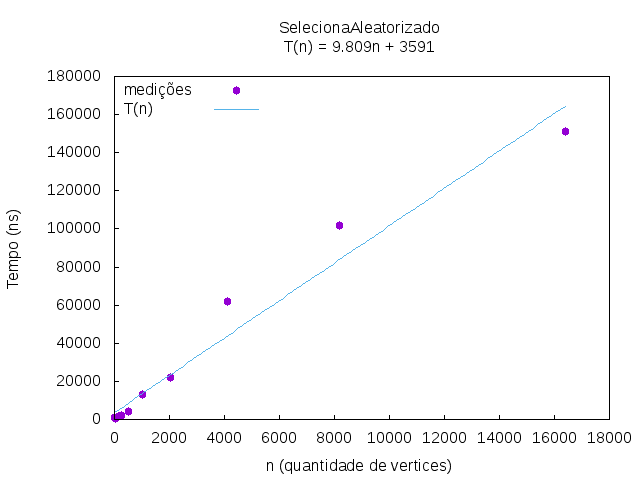
\includegraphics[width=0.7\linewidth]{graficos/SeletorRecursivoAtividades/Decrescente P40/SelecionaAleatorizado.png}
  \caption{Seleciona Recursivo de Atividade - Vetor decrescente P40}
\end{figure}




\subsection{Vetor Decrescente P50}
Tabela gerada utilizando Seleciona Recursivo de Atividade com vetores de tamanho n, sendo n = $(2^k)$, de k = 4..14 e inseridos Decrescente P50.
\begin{table}[H]
\centering
\caption{Seleciona Recursivo de Atividade com vetor decrescente P50}
\label{my-label}
\begin{tabular}{|l|l|}
\hline
\multicolumn{1}{|c|}{\textbf{Número de Elementos}} & \multicolumn{1}{c|}{\textbf{Tempo de execução em nanosegundos}} \\ \hline
16 & 593 \\ \hline
32 & 692 \\ \hline
64 & 1028 \\ \hline
128 & 2107 \\ \hline
256 & 3328 \\ \hline
512 & 5288 \\ \hline
1024 & 13776 \\ \hline
2048 & 26749 \\ \hline
4096 & 37678 \\ \hline
8192 & 112482 \\ \hline
16384 & 260308 \\ \hline
\end{tabular}
\end{table}

\begin{figure}[H]
    \centering
    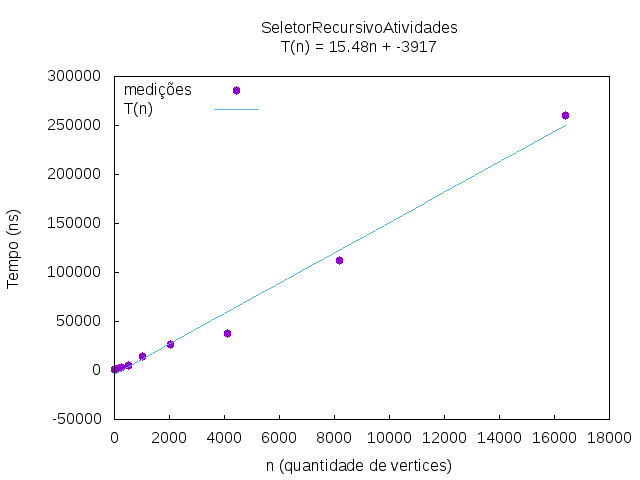
\includegraphics[width=0.7\linewidth]{graficos/SeletorRecursivoAtividades/Decrescente P50/SelecionaAleatorizado.png}
  \caption{Seleciona Recursivo de Atividade - Vetor decrescente P50}
\end{figure}


\section{Mochila Fracionaria}

Esse problema também é chamado problema da mochila 0/1 pois para
cada item deve ser levado ou deixado e pode-se pegar uma parte
fracionária de um item ou pegar um mesmo item mais que uma vez.

\subsection{Vetor ordenado}
Tabela gerada utilizando Mochila Fracionaria com Vetor ordenado de tamanho n, sendo n = $(2^k)$, de k = 4..14 e inseridos ordenada.
\begin{table}[H]
\centering
\caption{Mochila Fracionaria com vetor ordenado}
\label{my-label}
\begin{tabular}{|l|l|}
\hline
\multicolumn{1}{|c|}{\textbf{Número de Elementos}} & \multicolumn{1}{c|}{\textbf{Tempo de execução em nanosegundos}} \\ \hline
16 & 608 \\ \hline
32 & 699 \\ \hline
64 & 759 \\ \hline
128 & 770 \\ \hline
256 & 796 \\ \hline
512 & 830 \\ \hline
1024 & 949 \\ \hline
2048 & 1190 \\ \hline
4096 & 1565 \\ \hline
8192 & 2253 \\ \hline
16384 & 4106 \\ \hline
\end{tabular}
\end{table}

\begin{figure}[H]
    \centering
    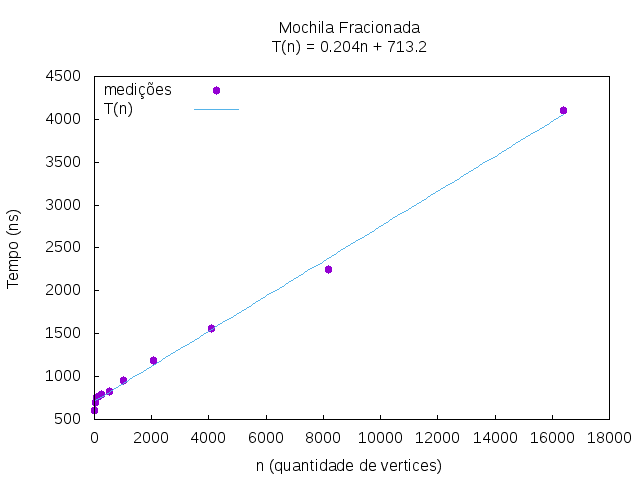
\includegraphics[width=0.7\linewidth]{graficos/Mochila Fracionada/MochilaFracionada.png}
  \caption{Mochila Fracionaria - Vetor ordenado}
\end{figure}


\chapter{Programação Dinâmica}

Programação dinâmica é um método para a construção de algoritmos para a resolução de problemas computacionais, em especial os de otimização combinatória. Ela é aplicável a problemas nos quais a solução ótima pode ser computada a partir da solução ótima previamente calculada e memorizada.

\section{Corte Haste}

O problema consiste em dada uma haste de npolegadas de comprimento, e uma tabela de preços pi, para i= 1,2,...,n, determinar qual a receita máxima que se pode obter cortando a haste e vendendo os seus pedaços, considerando que os comprimentos são sempre números inteiros de polegadas.


\section{Corte Haste Bottom Up}

É uma aproximação do problema de Corte de Haste utilizando a arvore de Bottom Up.

\subsection{Vetor aleatorio}
Tabela gerada utilizando Corte Haste Bottom Up com vetores de tamanho n, sendo n = $(2^k)$, de k = 4..14 e inseridos aleatóriamente.
\begin{table}[H]
\centering
\caption{Corte Haste Bottom Up com vetor aleatório}
\label{my-label}
\begin{tabular}{|l|l|}
\hline
\multicolumn{1}{|c|}{\textbf{Número de Elementos}} & \multicolumn{1}{c|}{\textbf{Tempo de execução em nanosegundos}} \\ \hline
16 & 599 \\ \hline
32 & 913 \\ \hline
64 & 1798 \\ \hline
128 & 4618 \\ \hline
256 & 14530 \\ \hline
512 & 51214 \\ \hline
1024 & 193794 \\ \hline
2048 & 761470 \\ \hline
4096 & 2965012 \\ \hline
8192 & 12774326 \\ \hline
16384 & 48066532 \\ \hline
\end{tabular}
\end{table}

\begin{figure}[H]
    \centering
    \includegraphics[width=0.7\linewidth]{graficos/CorteHasteBottomUp/HasteBU.png}
  \caption{Corte Haste Bottom Up - Vetor Aleatório}
\end{figure}

\section{Corte Haste Comum}

Refere ao problema já mencionado anteriormente.

\subsection{Vetor Comum}
Vetores menores devido a estouro de memória.
\begin{table}[H]
\centering
\caption{Corte Haste Bottom Up com vetor aleatório}
\label{my-label}
\begin{tabular}{|l|l|}
\hline
\multicolumn{1}{|c|}{\textbf{Número de Elementos}} & \multicolumn{1}{c|}{\textbf{Tempo de execução em nanosegundos}} \\ \hline
1 & 130 \\ \hline
2 & 261 \\ \hline
3 & 522 \\ \hline
4 & 1045 \\ \hline
5 & 2091 \\ \hline
6 & 4182 \\ \hline
7 & 8365 \\ \hline
8 & 16731 \\ \hline
9 & 33463 \\ \hline
10 & 66926 \\ \hline
11 & 133852 \\ \hline
12 & 267705 \\ \hline
16 & 535410 \\ \hline
\end{tabular}
\end{table}
\begin{figure}[H]
    \centering
    \includegraphics[width=0.7\linewidth]{graficos/CorteHasteComum/HasteBU.png}
  \caption{Corte Haste Comum - Vetor Aleatório}
\end{figure}

\section{Corte Haste Memoizada}

É uma aproximação do algoritmo utilizando a arvore Top DowN.

\subsection{Vetor aleatorio}
Tabela gerada utilizando Corte Haste Memoizada com vetores de tamanho n, sendo n = $(2^k)$, de k = 4..14 e inseridos aleatóriamente.
\begin{table}[H]
\centering
\caption{Corte Haste Memoizada com vetor aleatório}
\label{my-label}
\begin{tabular}{|l|l|}
\hline
\multicolumn{1}{|c|}{\textbf{Número de Elementos}} & \multicolumn{1}{c|}{\textbf{Tempo de execução em nanosegundos}} \\ \hline
16 & 1285 \\ \hline
32 & 323 \\ \hline
64 & 325 \\ \hline
128 & 296 \\ \hline
256 & 334 \\ \hline
512 & 376 \\ \hline
1024 & 545 \\ \hline
2048 & 1325 \\ \hline
4096 & 2331 \\ \hline
8192 & 3844 \\ \hline
16384 & 15475 \\ \hline
\end{tabular}
\end{table}

\begin{figure}[H]
    \centering
    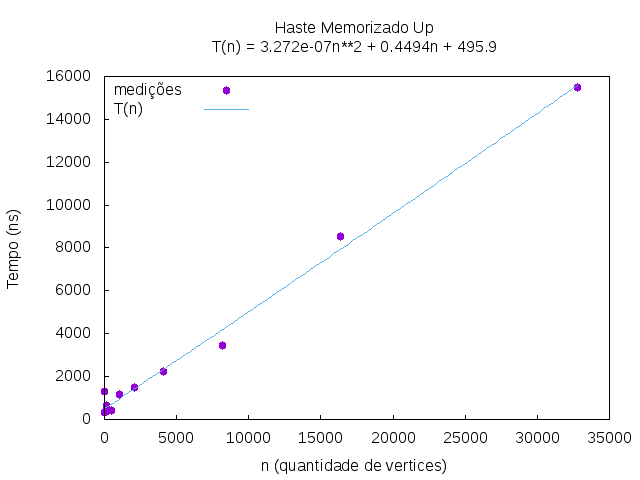
\includegraphics[width=0.7\linewidth]{graficos/CorteHasteMemorizado/Aleatorio/HasteMemo.png}
  \caption{Corte Haste Memoizada - Vetor Aleatório}
\end{figure}

\subsection{Vetor Crescente P10}
Tabela gerada utilizando Corte Haste Memoizada com vetores de tamanho n, sendo n = $(2^k)$, de k = 4..14 e inseridos de forma crescente P10.
\begin{table}[H]
\centering
\caption{Corte Haste Memoizada com Vetor Crescente P10}
\label{my-label}
\begin{tabular}{|l|l|}
\hline
\multicolumn{1}{|c|}{\textbf{Número de Elementos}} & \multicolumn{1}{c|}{\textbf{Tempo de execução em nanosegundos}} \\ \hline
16 & 1398 \\ \hline
32 & 3456 \\ \hline
64 & 6795 \\ \hline
128 & 12053 \\ \hline
256 & 24546 \\ \hline
512 & 48256 \\ \hline
1024 & 90413 \\ \hline
2048 & 180521 \\ \hline
4096 & 360512 \\ \hline
8192 & 808256 \\ \hline
16384 & 6200211 \\ \hline
\end{tabular}
\end{table}

\begin{figure}[H]
    \centering
    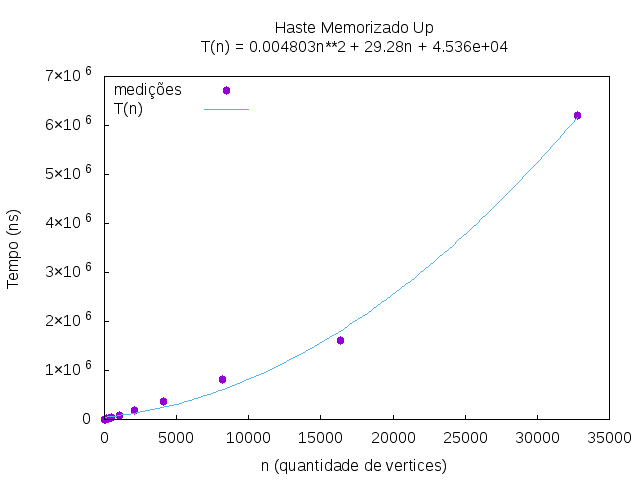
\includegraphics[width=0.7\linewidth]{graficos/CorteHasteMemorizado/CrescenteP10/HasteMemo.png}
  \caption{Corte Haste Memoizada - Vetor Crescente P10}
\end{figure}

\subsection{Vetor Crescente P20}
Tabela gerada utilizando Corte Haste Memoizada com vetores de tamanho n, sendo n = $(2^k)$, de k = 4..14 e inseridos de forma crescente P20.
\begin{table}[H]
\centering
\caption{Corte Haste Memoizada com Vetor Crescente P20}
\label{my-label}
\begin{tabular}{|l|l|}
\hline
\multicolumn{1}{|c|}{\textbf{Número de Elementos}} & \multicolumn{1}{c|}{\textbf{Tempo de execução em nanosegundos}} \\ \hline
16 & 360 \\ \hline
32 & 338 \\ \hline
64 & 388 \\ \hline
128 & 472 \\ \hline
256 & 393 \\ \hline
512 & 525 \\ \hline
1024 & 619 \\ \hline
2048 & 1236 \\ \hline
4096 & 1041 \\ \hline
8192 & 1519 \\ \hline
16384 & 3379 \\ \hline

\end{tabular}
\end{table}

\begin{figure}[H]
    \centering
    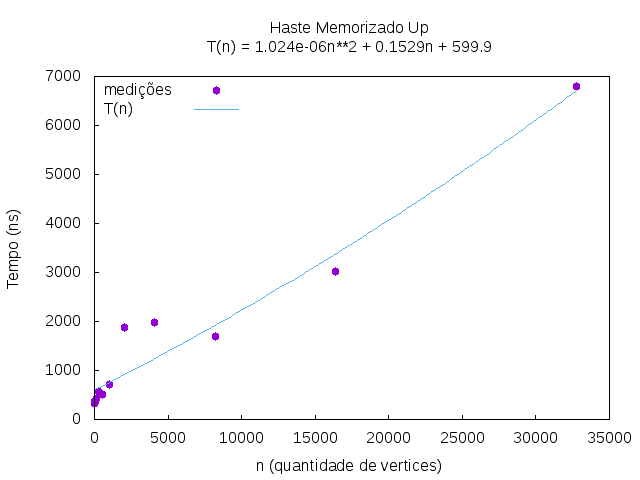
\includegraphics[width=0.7\linewidth]{graficos/CorteHasteMemorizado/CrescenteP20/HasteMemo.png}
  \caption{Corte Haste Memoizada - Vetor Crescente P20}
\end{figure}



\subsection{Vetor Crescente P30}
Tabela gerada utilizando Corte Haste Memoizada com vetores de tamanho n, sendo n = $(2^k)$, de k = 4..14 e inseridos de forma crescente P30.
\begin{table}[H]
\centering
\caption{Corte Haste Memoizada com Vetor Crescente P30}
\label{my-label}
\begin{tabular}{|l|l|}
\hline
\multicolumn{1}{|c|}{\textbf{Número de Elementos}} & \multicolumn{1}{c|}{\textbf{Tempo de execução em nanosegundos}} \\ \hline
16 & 373 \\ \hline
32 & 369 \\ \hline
64 & 396 \\ \hline
128 & 386 \\ \hline
256 & 618 \\ \hline
512 & 667 \\ \hline
1024 & 1786 \\ \hline
2048 & 2808 \\ \hline
4096 & 3943 \\ \hline
8192 & 6857 \\ \hline
16384 & 16596 \\ \hline
\end{tabular}
\end{table}

\begin{figure}[H]
    \centering
    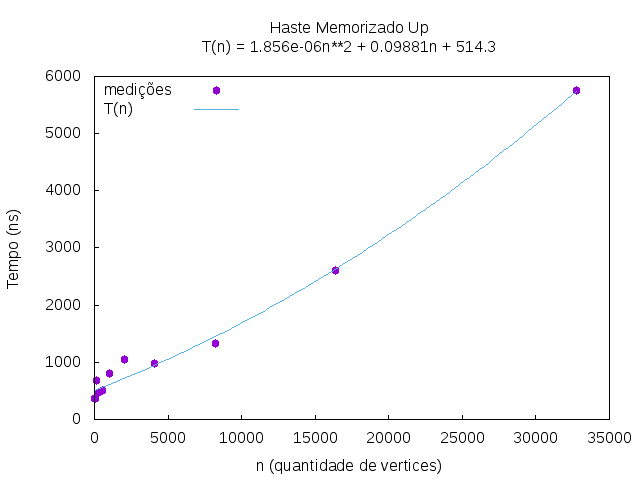
\includegraphics[width=0.7\linewidth]{graficos/CorteHasteMemorizado/CrescenteP30/HasteMemo.png}
  \caption{Corte Haste Memoizada - Vetor Crescente P30}
\end{figure}





\subsection{Vetor Crescente P40}
Tabela gerada utilizando Corte Haste Memoizada com vetores de tamanho n, sendo n = $(2^k)$, de k = 4..14 e inseridos de forma crescente P40.
\begin{table}[H]
\centering
\caption{Corte Haste Memoizada com Vetor Crescente P40}
\label{my-label}
\begin{tabular}{|l|l|}
\hline
\multicolumn{1}{|c|}{\textbf{Número de Elementos}} & \multicolumn{1}{c|}{\textbf{Tempo de execução em nanosegundos}} \\ \hline
16 & 485 \\ \hline
32 & 480 \\ \hline
64 & 563 \\ \hline
128 & 836 \\ \hline
256 & 707 \\ \hline
512 & 710 \\ \hline
1024 & 483 \\ \hline
2048 & 680 \\ \hline
4096 & 1127 \\ \hline
8192 & 1849 \\ \hline
16384 & 3551 \\ \hline
\end{tabular}
\end{table}

\begin{figure}[H]
    \centering
    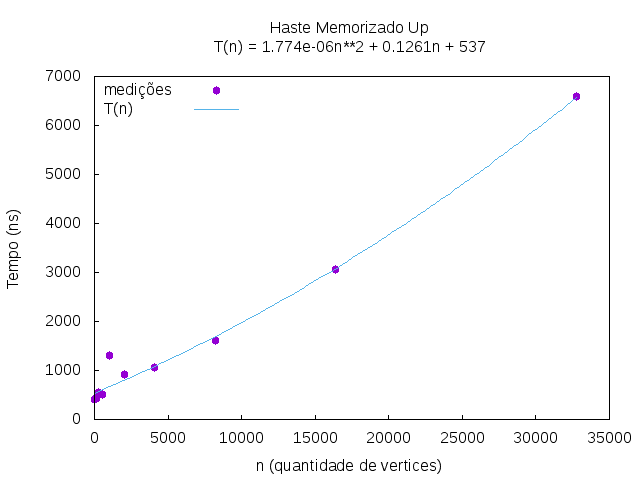
\includegraphics[width=0.7\linewidth]{graficos/CorteHasteMemorizado/CrescenteP40/HasteMemo.png}
  \caption{Corte Haste Memoizada - Vetor Crescente P40}
\end{figure}




\subsection{Vetor Crescente P50}
Tabela gerada utilizando Corte Haste Memoizada com vetores de tamanho n, sendo n = $(2^k)$, de k = 4..14 e inseridos de forma crescente P50.
\begin{table}[H]
\centering
\caption{Corte Haste Memoizada com Vetor Crescente P50}
\label{my-label}
\begin{tabular}{|l|l|}
\hline
\multicolumn{1}{|c|}{\textbf{Número de Elementos}} & \multicolumn{1}{c|}{\textbf{Tempo de execução em nanosegundos}} \\ \hline
16 & 473 \\ \hline
32 & 401 \\ \hline
64 & 801 \\ \hline
128 & 995 \\ \hline
256 & 821 \\ \hline
512 & 405 \\ \hline
1024 & 681 \\ \hline
2048 & 720 \\ \hline
4096 & 1075 \\ \hline
8192 & 1818 \\ \hline
16384 & 3658 \\ \hline
\end{tabular}
\end{table}

\begin{figure}[H]
    \centering
    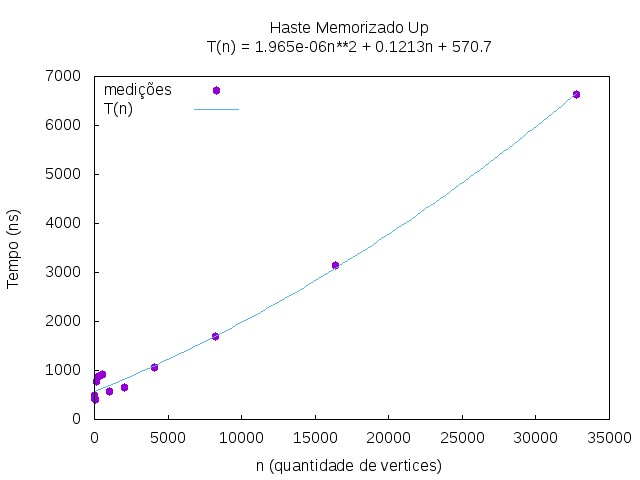
\includegraphics[width=0.7\linewidth]{graficos/CorteHasteMemorizado/Crescente50/HasteMemo.png}
  \caption{Corte Haste Memoizada - Vetor Crescente P50}
\end{figure}


\subsection{Vetor Decrescente}
Tabela gerada utilizando Corte Haste Memoizada com vetores de tamanho n, sendo n = $(2^k)$, de k = 4..14 e inseridos de forma decrescente.
\begin{table}[H]
\centering
\caption{Corte Haste Memoizada com Vetor Decrescente}
\label{my-label}
\begin{tabular}{|l|l|}
\hline
\multicolumn{1}{|c|}{\textbf{Número de Elementos}} & \multicolumn{1}{c|}{\textbf{Tempo de execução em nanosegundos}} \\ \hline
16 & 1598 \\ \hline
32 & 3256 \\ \hline
64 & 5795 \\ \hline
128 & 12196 \\ \hline
256 & 24649 \\ \hline
512 & 48146 \\ \hline
1024 & 91564 \\ \hline
2048 & 183545 \\ \hline
4096 & 335949 \\ \hline
8192 & 815698 \\ \hline
16384 & 6198565 \\ \hline
\end{tabular}
\end{table}

\begin{figure}[H]
    \centering
    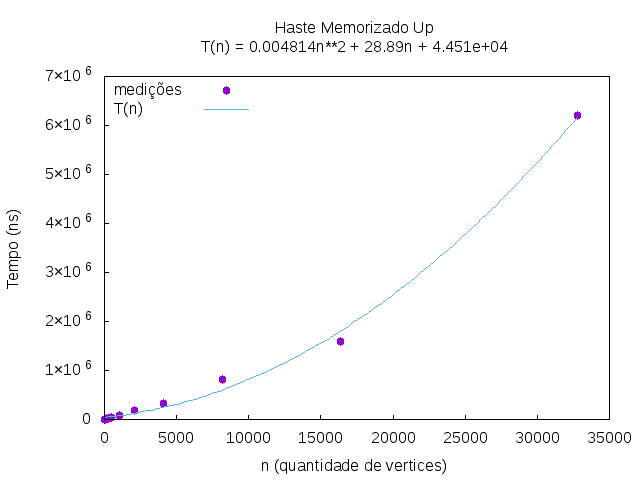
\includegraphics[width=0.7\linewidth]{graficos/CorteHasteMemorizado/Decrescente/HasteMemo.png}
  \caption{Corte Haste Memoizada - Vetor Decrescente}
\end{figure}


\subsection{Vetor Decrescente P10}
Tabela gerada utilizando Corte Haste Memoizada com vetores de tamanho n, sendo n = $(2^k)$, de k = 4..14 e inseridos de forma decrescente P10.
\begin{table}[H]
\centering
\caption{Corte Haste Memoizada com Vetor Decrescente P10}
\label{my-label}
\begin{tabular}{|l|l|}
\hline
\multicolumn{1}{|c|}{\textbf{Número de Elementos}} & \multicolumn{1}{c|}{\textbf{Tempo de execução em nanosegundos}} \\ \hline
16 & 1398 \\ \hline
32 & 2956 \\ \hline
64 & 5465 \\ \hline
128 & 13196 \\ \hline
256 & 25697 \\ \hline
512 & 50154 \\ \hline
1024 & 93484 \\ \hline
2048 & 183654 \\ \hline
4096 & 315169 \\ \hline
8192 & 835495 \\ \hline
16384 & 1588859 \\ \hline

\end{tabular}
\end{table}

\begin{figure}[H]
    \centering
    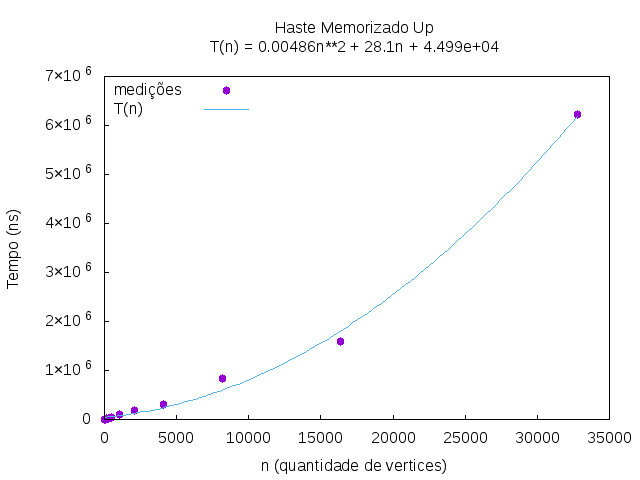
\includegraphics[width=0.7\linewidth]{graficos/CorteHasteMemorizado/DecrescenteP10/HasteMemo.png}
  \caption{Corte Haste Memoizada - Vetor Decrescente P10}
\end{figure}

\subsection{Vetor Decrescente P20}
Tabela gerada utilizando Corte Haste Memoizada com vetores de tamanho n, sendo n = $(2^k)$, de k = 4..14 e inseridos de forma decrescente P20.
\begin{table}[H]
\centering
\caption{Corte Haste Memoizada com Vetor Decrescente P20}
\label{my-label}
\begin{tabular}{|l|l|}
\hline
\multicolumn{1}{|c|}{\textbf{Número de Elementos}} & \multicolumn{1}{c|}{\textbf{Tempo de execução em nanosegundos}} \\ \hline
16 & 726 \\ \hline
32 & 2229 \\ \hline
64 & 633 \\ \hline
128 & 633 \\ \hline
256 & 1107 \\ \hline
512 & 736 \\ \hline
1024 & 1011 \\ \hline
2048 & 1372 \\ \hline
4096 & 2078 \\ \hline
8192 & 3247 \\ \hline
16384 & 6265 \\ \hline

\end{tabular}
\end{table}

\begin{figure}[H]
    \centering
    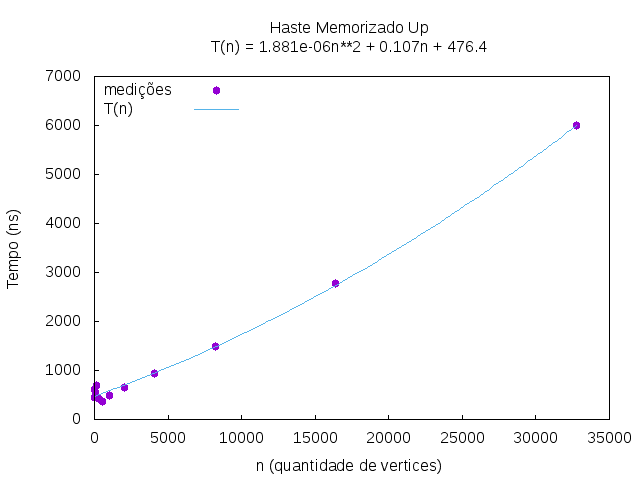
\includegraphics[width=0.7\linewidth]{graficos/CorteHasteMemorizado/DecrescenteP20/HasteMemo.png}
  \caption{Corte Haste Memoizada - Vetor Decrescente P20}
\end{figure}



\subsection{Vetor Decrescente P30}
Tabela gerada utilizando Corte Haste Memoizada com vetores de tamanho n, sendo n = $(2^k)$, de k = 4..14 e inseridos de forma decrescente P30.
\begin{table}[H]
\centering
\caption{Corte Haste Memoizada com Vetor Decrescente P30}
\label{my-label}
\begin{tabular}{|l|l|}
\hline
\multicolumn{1}{|c|}{\textbf{Número de Elementos}} & \multicolumn{1}{c|}{\textbf{Tempo de execução em nanosegundos}} \\ \hline
16 & 701 \\ \hline
32 & 337 \\ \hline
64 & 350 \\ \hline
128 & 367 \\ \hline
256 & 365 \\ \hline
512 & 631 \\ \hline
1024 & 493 \\ \hline
2048 & 803 \\ \hline
4096 & 1145 \\ \hline
8192 & 2082 \\ \hline
16384 & 4729 \\ \hline

\end{tabular}
\end{table}

\begin{figure}[H]
    \centering
    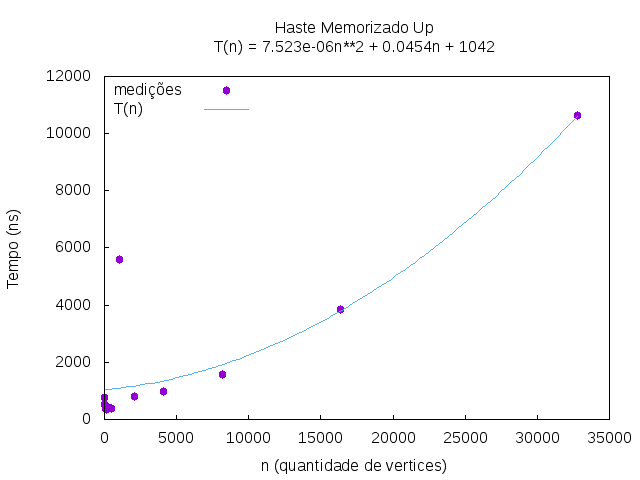
\includegraphics[width=0.7\linewidth]{graficos/CorteHasteMemorizado/DecrescenteP30/HasteMemo.png}
  \caption{Corte Haste Memoizada - Vetor Decrescente P30}
\end{figure}




\subsection{Vetor Decrescente P40}
Tabela gerada utilizando Corte Haste Memoizada com vetores de tamanho n, sendo n = $(2^k)$, de k = 4..14 e inseridos de forma decrescente P40.
\begin{table}[H]
\centering
\caption{Corte Haste Memoizada com Vetor Decrescente P40}
\label{my-label}
\begin{tabular}{|l|l|}
\hline
\multicolumn{1}{|c|}{\textbf{Número de Elementos}} & \multicolumn{1}{c|}{\textbf{Tempo de execução em nanosegundos}} \\ \hline
16 & 357 \\ \hline
32 & 362 \\ \hline
64 & 364 \\ \hline
128 & 372 \\ \hline
256 & 392 \\ \hline
512 & 427 \\ \hline
1024 & 545 \\ \hline
2048 & 604 \\ \hline
4096 & 1085 \\ \hline
8192 & 13662 \\ \hline
16384 & 16253 \\ \hline

\end{tabular}
\end{table}

\begin{figure}[H]
    \centering
    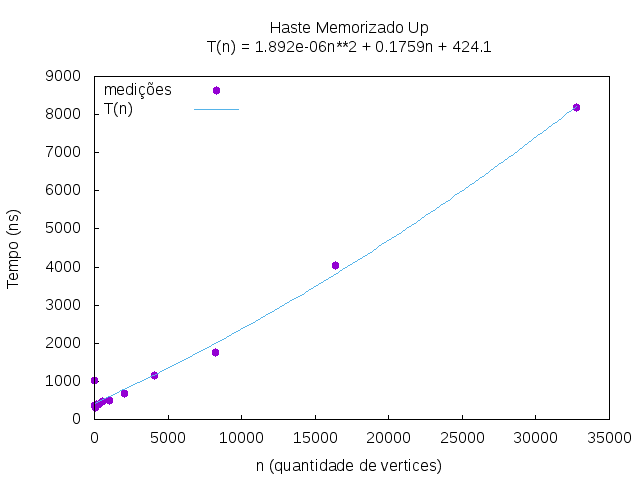
\includegraphics[width=0.7\linewidth]{graficos/CorteHasteMemorizado/DecrescenteP40/HasteMemo.png}
  \caption{Corte Haste Memoizada - Vetor Decrescente P40}
\end{figure}


\subsection{Vetor Decrescente P50}
Tabela gerada utilizando Corte Haste Memoizada com vetores de tamanho n, sendo n = $(2^k)$, de k = 4..14 e inseridos de forma decrescente P50.
\begin{table}[H]
\centering
\caption{Corte Haste Memoizada com Vetor Decrescente P50}
\label{my-label}
\begin{tabular}{|l|l|}
\hline
\multicolumn{1}{|c|}{\textbf{Número de Elementos}} & \multicolumn{1}{c|}{\textbf{Tempo de execução em nanosegundos}} \\ \hline
16 & 372 \\ \hline
32 & 650 \\ \hline
64 & 1251 \\ \hline
128 & 2654 \\ \hline
256 & 5659 \\ \hline
512 & 11256 \\ \hline
1024 & 20265 \\ \hline
2048 & 35654 \\ \hline
4096 & 71565 \\ \hline
8192 & 156984 \\ \hline
16384 & 305465 \\ \hline
\end{tabular}
\end{table}

\begin{figure}[H]
    \centering
    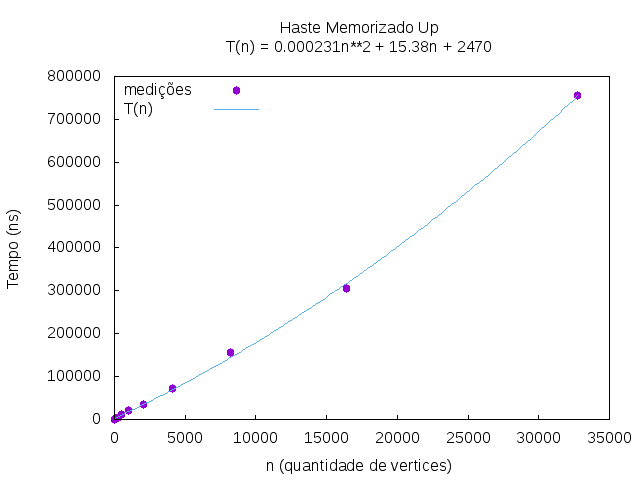
\includegraphics[width=0.7\linewidth]{graficos/CorteHasteMemorizado/DecrescenteP50/HasteMemo.png}
  \caption{Corte Haste Memoizada - Vetor Decrescente P50}
\end{figure}

\section{SCM}

Suponha que A[1..n] é uma sequência de números naturais. Uma subsequência de A[1..n] é o que sobra depois que um conjunto arbitrário de termos é apagado.  (Não confunda subsequência com segmento: um segmento de A[1..n] é o que sobra depois que apagamos um número arbitrário de termos no início de A e um número arbitrário de termos no fim de A).

\subsection{Vetor caracteres}
Tabela gerada utilizando SCM com vetores de tamanho n, sendo n = $(2^k)$, de k = 4..14.
\begin{table}[H]
\centering
\caption{SCM com vetor de caracteres}
\label{my-label}
\begin{tabular}{|l|l|}
\hline
\multicolumn{1}{|c|}{\textbf{Número de Elementos}} & \multicolumn{1}{c|}{\textbf{Tempo de execução em nanosegundos}} \\ \hline
16 & 7047 \\ \hline
32 & 12406 \\ \hline
64 & 23325 \\ \hline
128 & 53892 \\ \hline
256 & 111991 \\ \hline
512 & 181464 \\ \hline
1024 & 356165 \\ \hline
2048 & 708123 \\ \hline
4096 & 1434151 \\ \hline
8192 & 3129872 \\ \hline
16384 & 6078938 \\ \hline

\end{tabular}
\end{table}

\begin{figure}[H]
    \centering
    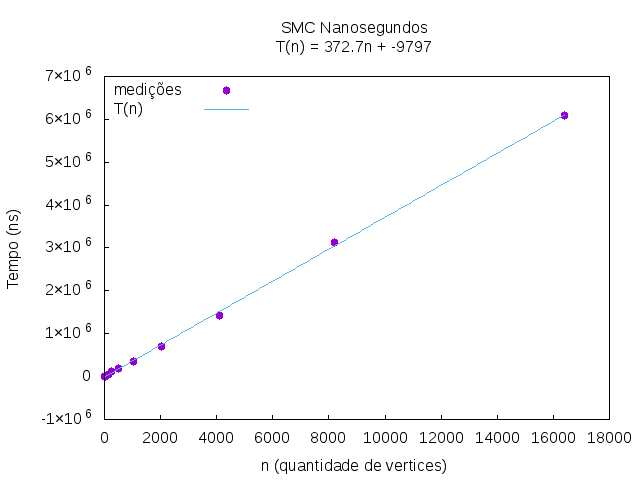
\includegraphics[width=0.7\linewidth]{graficos/SMC Nanosegundos/SMCNanosegundos.png}
  \caption{SCM - Vetor caracteres}
\end{figure}


\section{SCM Recursivo}

Problema já comentado anteriormente.

\subsection{Vetor caracteres}
Tabela gerada utilizando SCM Recursivo com vetores de tamanho n, sendo n = $(2^k)$, de k = 4..14.
Não foi possível retirar conclusões, pois estoura a pilha.
\begin{table}[H]
\centering
\caption{SCM Recursivo com vetor de caracteres}
\label{my-label}
\begin{tabular}{|l|l|}
\hline
\multicolumn{1}{|c|}{\textbf{Número de Elementos}} & \multicolumn{1}{c|}{\textbf{Tempo de execução em nanosegundos}} \\ \hline
10 & 1235274 \\ \hline
20 & 1273575975 \\ \hline
30 & 1080524745749 \\ \hline
\end{tabular}
\end{table}

\section{Parentização Bottom Up}

A forma com a qual a parentizamos uma cadeia de matrizes afeta dramaticamente o custo de calcular o produto. Problema resolvido com uma arvore Bottom Up.

\subsection{Vetor aleatorio}
Tabela gerada utilizando Parentização Bottom Up com vetores de tamanho n, sendo n = $(2^k)$, de k = 4..14 e inseridos aleatóriamente.
\begin{table}[H]
\centering
\caption{Parentização Bottom Up com vetor aleatório}
\label{my-label}
\begin{tabular}{|l|l|}
\hline
\multicolumn{1}{|c|}{\textbf{Número de Elementos}} & \multicolumn{1}{c|}{\textbf{Tempo de execução em nanosegundos}} \\ \hline
16 & 3216 \\ \hline
32 & 19174 \\ \hline
64 & 118943 \\ \hline
128 & 866385 \\ \hline
256 & 6978135 \\ \hline
512 & 69493017 \\ \hline
\end{tabular}
\end{table}

\begin{figure}[H]
    \centering
    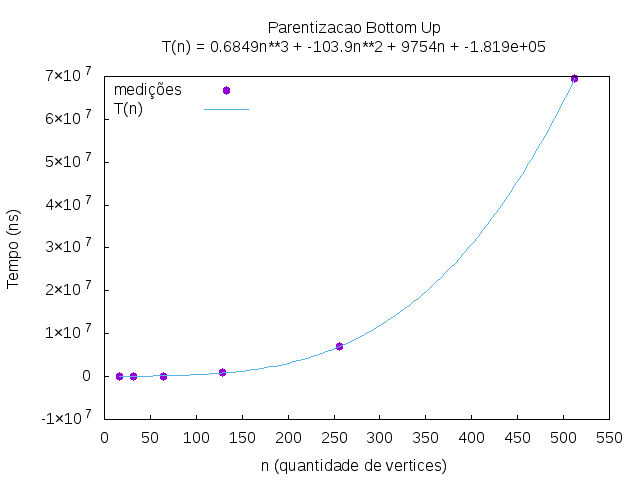
\includegraphics[width=0.7\linewidth]{graficos/Parentizacao BottomUp/Aleatorio/ParentizacaoBottomUp.png}
  \caption{Parentização Bottom Up - Vetor Aleatório}
\end{figure}



\subsection{Vetor Crescente}
Tabela gerada utilizando Parentização Bottom Up com vetores de tamanho n, sendo n = $(2^
k)$, de k = 4..14 e inseridos Crescente.
\begin{table}[H]
\centering
\caption{Parentização Bottom Up com vetor Crescente}
\label{my-label}
\begin{tabular}{|l|l|}
\hline
\multicolumn{1}{|c|}{\textbf{Número de Elementos}} & \multicolumn{1}{c|}{\textbf{Tempo de execução em nanosegundos}} \\ \hline
16 & 2552 \\ \hline
32 & 13783 \\ \hline
64 & 93670 \\ \hline
128 & 746015 \\ \hline
256 & 6597644 \\ \hline
512 & 67582370 \\ \hline
\end{tabular}
\end{table}

\begin{figure}[H]
    \centering
    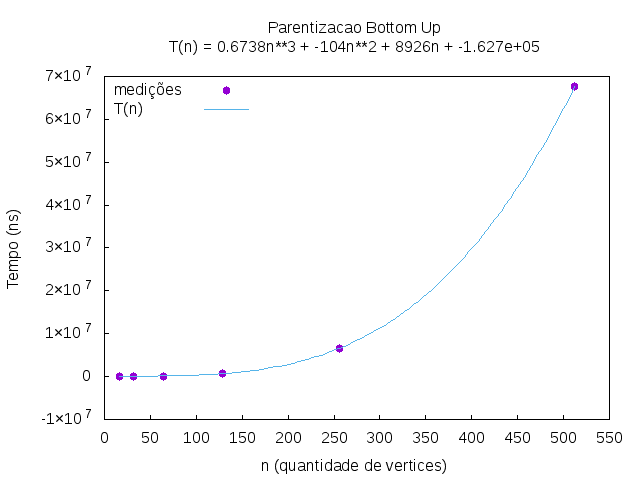
\includegraphics[width=0.7\linewidth]{graficos/Parentizacao BottomUp/Crescente/ParentizacaoBottomUp.png}
  \caption{Parentização Bottom Up - Vetor Crescente}
\end{figure}


\subsection{Vetor Crescente P10}
Tabela gerada utilizando Parentização Bottom Up com vetores de tamanho n, sendo n = $(2^k)$, de k = 4..14 e inseridos Crescente P10.
\begin{table}[H]
\centering
\caption{Parentização Bottom Up com vetor Crescente P10}
\label{my-label}
\begin{tabular}{|l|l|}
\hline
\multicolumn{1}{|c|}{\textbf{Número de Elementos}} & \multicolumn{1}{c|}{\textbf{Tempo de execução em nanosegundos}} \\ \hline
16 & 2467 \\ \hline
32 & 13724 \\ \hline
64 & 92732 \\ \hline
128 & 743649 \\ \hline
256 & 6495094 \\ \hline
512 & 67519336 \\ \hline
\end{tabular}
\end{table}

\begin{figure}[H]
    \centering
    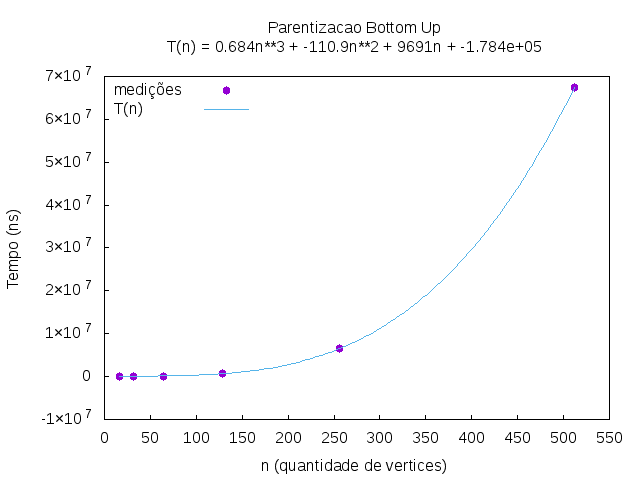
\includegraphics[width=0.7\linewidth]{graficos/Parentizacao BottomUp/Crescente P10/ParentizacaoBottomUp.png}
  \caption{Parentização Bottom Up - Vetor Crescente P10}
\end{figure}




\subsection{Vetor Crescente P20}
Tabela gerada utilizando Parentização Bottom Up com vetores de tamanho n, sendo n = $(2^k)$, de k = 4..14 e inseridos Crescente P20.
\begin{table}[H]
\centering
\caption{Parentização Bottom Up com vetor Crescente P20}
\label{my-label}
\begin{tabular}{|l|l|}
\hline
\multicolumn{1}{|c|}{\textbf{Número de Elementos}} & \multicolumn{1}{c|}{\textbf{Tempo de execução em nanosegundos}} \\ \hline
16 & 2413 \\ \hline
32 & 14015 \\ \hline
64 & 97281 \\ \hline
128 & 723129 \\ \hline
256 & 6471911 \\ \hline
512 & 67329970 \\ \hline
\end{tabular}
\end{table}

\begin{figure}[H]
    \centering
    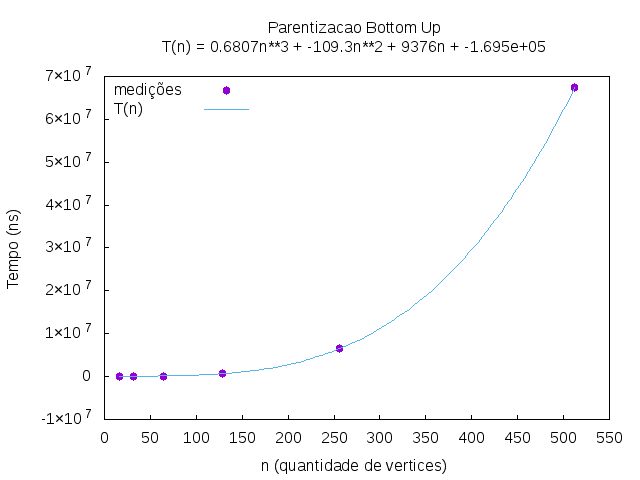
\includegraphics[width=0.7\linewidth]{graficos/Parentizacao BottomUp/Crescente P20/ParentizacaoBottomUp.png}
  \caption{Parentização Bottom Up - Vetor Crescente P20}
\end{figure}


\subsection{Vetor Crescente P30}
Tabela gerada utilizando Parentização Bottom Up com vetores de tamanho n, sendo n = $(2^k)$, de k = 4..14 e inseridos Crescente P30.
\begin{table}[H]
\centering
\caption{Parentização Bottom Up com vetor Crescente P30}
\label{my-label}
\begin{tabular}{|l|l|}
\hline
\multicolumn{1}{|c|}{\textbf{Número de Elementos}} & \multicolumn{1}{c|}{\textbf{Tempo de execução em nanosegundos}} \\ \hline
16 & 2446 \\ \hline
32 & 14459 \\ \hline
64 & 96241 \\ \hline
128 & 731624 \\ \hline
256 & 6419155 \\ \hline
512 & 67127224 \\ \hline
\end{tabular}
\end{table}

\begin{figure}[H]
    \centering
    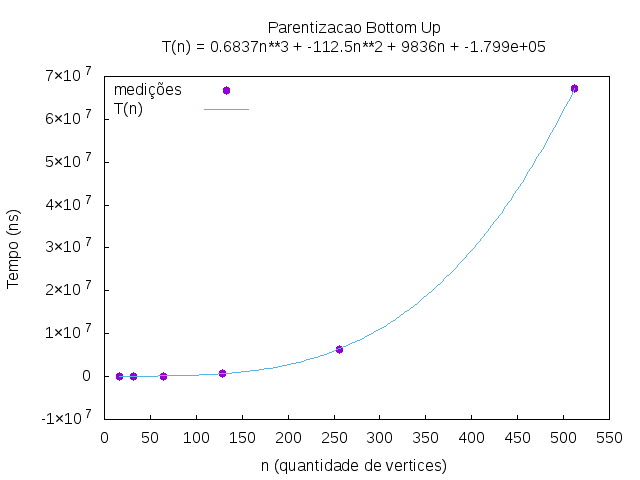
\includegraphics[width=0.7\linewidth]{graficos/Parentizacao BottomUp/Crescente P30/ParentizacaoBottomUp.png}
  \caption{Parentização Bottom Up - Vetor Crescente P30}
\end{figure}

\subsection{Vetor Crescente P40}
Tabela gerada utilizando Parentização Bottom Up com vetores de tamanho n, sendo n = $(2^k)$, de k = 4..14 e inseridos Crescente P40.
\begin{table}[H]
\centering
\caption{Parentização Bottom Up com vetor Crescente P40}
\label{my-label}
\begin{tabular}{|l|l|}
\hline
\multicolumn{1}{|c|}{\textbf{Número de Elementos}} & \multicolumn{1}{c|}{\textbf{Tempo de execução em nanosegundos}} \\ \hline
16 & 2475 \\ \hline
32 & 14317 \\ \hline
64 & 99423 \\ \hline
128 & 738641 \\ \hline
256 & 6484759 \\ \hline
512 & 67394010 \\ \hline

\end{tabular}
\end{table}

\begin{figure}[H]
    \centering
    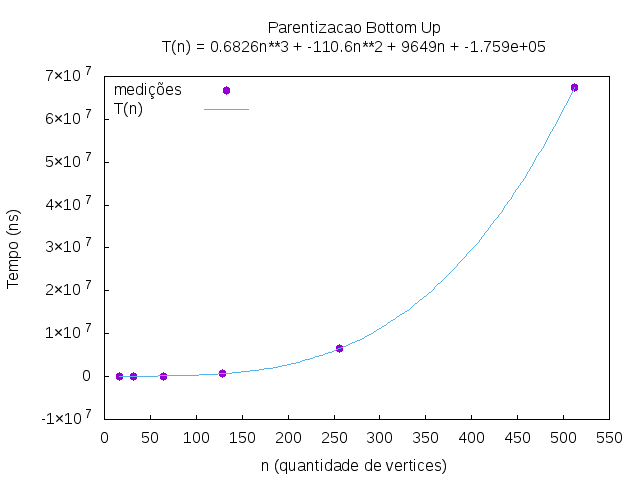
\includegraphics[width=0.7\linewidth]{graficos/Parentizacao BottomUp/Crescente P40/ParentizacaoBottomUp.png}
  \caption{Parentização Bottom Up - Vetor Crescente P40}
\end{figure}

\subsection{Vetor Crescente P50}
Tabela gerada utilizando Parentização Bottom Up com vetores de tamanho n, sendo n = $(2^k)$, de k = 4..14 e inseridos Crescente P50.
\begin{table}[H]
\centering
\caption{Parentização Bottom Up com vetor Crescente P50}
\label{my-label}
\begin{tabular}{|l|l|}
\hline
\multicolumn{1}{|c|}{\textbf{Número de Elementos}} & \multicolumn{1}{c|}{\textbf{Tempo de execução em nanosegundos}} \\ \hline
16 & 3150 \\ \hline
32 & 13708 \\ \hline
64 & 93130 \\ \hline
128 & 727210 \\ \hline
256 & 6487127 \\ \hline
512 & 67246806 \\ \hline
\end{tabular}
\end{table}

\begin{figure}[H]
    \centering
    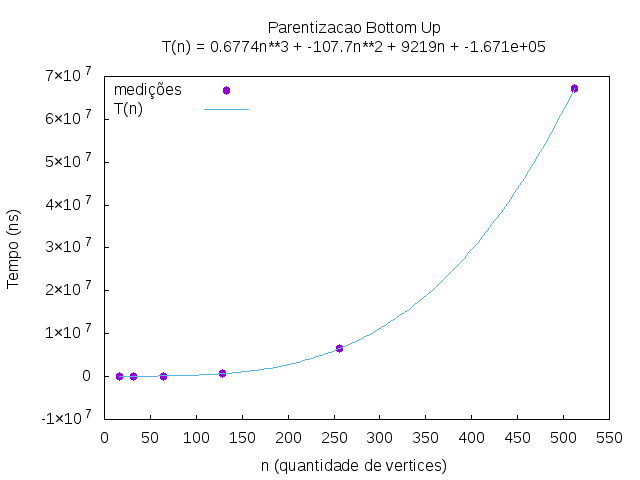
\includegraphics[width=0.7\linewidth]{graficos/Parentizacao BottomUp/Crescente P50/ParentizacaoBottomUp.png}
  \caption{Parentização Bottom Up - Vetor Crescente P50}
\end{figure}

\subsection{Vetor Decrescente}
Tabela gerada utilizando Parentização Bottom Up com vetores de tamanho n, sendo n = $(2^k)$, de k = 4..14 e inseridos Decrescente.
\begin{table}[H]
\centering
\caption{Parentização Bottom Up com vetor Decrescente}
\label{my-label}
\begin{tabular}{|l|l|}
\hline
\multicolumn{1}{|c|}{\textbf{Número de Elementos}} & \multicolumn{1}{c|}{\textbf{Tempo de execução em nanosegundos}} \\ \hline
16 & 2230 \\ \hline
32 & 11873 \\ \hline
64 & 94244 \\ \hline
128 & 690616 \\ \hline
256 & 6290244 \\ \hline
512 & 67357198 \\ \hline
\end{tabular}
\end{table}

\begin{figure}[H]
    \centering
    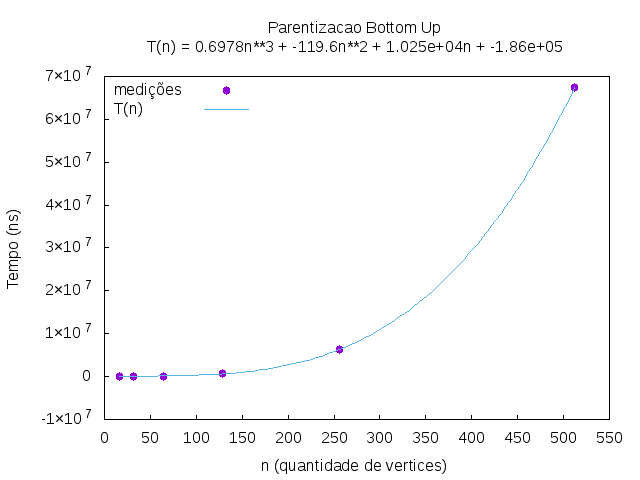
\includegraphics[width=0.7\linewidth]{graficos/Parentizacao BottomUp/Decrescente/ParentizacaoBottomUp.png}
  \caption{Parentização Bottom Up - Vetor Decrescente}
\end{figure}

\subsection{Vetor Decrescente P10}
Tabela gerada utilizando Parentização Bottom Up com vetores de tamanho n, sendo n = $(2^k)$, de k = 4..14 e inseridos Decrescente P10.
\begin{table}[H]
\centering
\caption{Parentização Bottom Up com vetor Decrescente P10}
\label{my-label}
\begin{tabular}{|l|l|}
\hline
\multicolumn{1}{|c|}{\textbf{Número de Elementos}} & \multicolumn{1}{c|}{\textbf{Tempo de execução em nanosegundos}} \\ \hline
16 & 3662 \\ \hline
32 & 13509 \\ \hline
64 & 104326 \\ \hline
128 & 723638 \\ \hline
256 & 6348032 \\ \hline
512 & 66932636 \\ \hline

\end{tabular}
\end{table}

\begin{figure}[H]
    \centering
    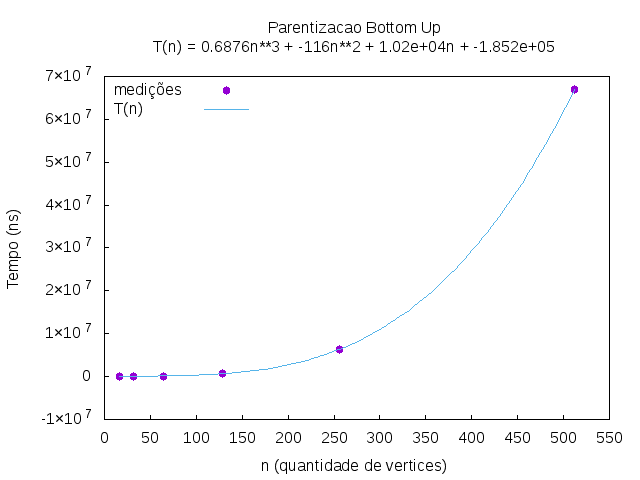
\includegraphics[width=0.7\linewidth]{graficos/Parentizacao BottomUp/Decrescente P10/ParentizacaoBottomUp.png}
  \caption{Parentização Bottom Up - Vetor Decrescente P10}
\end{figure}


\subsection{Vetor Decrescente P20}
Tabela gerada utilizando Parentização Bottom Up com vetores de tamanho n, sendo n = $(2^k)$, de k = 4..14 e inseridos Decrescente P20.
\begin{table}[H]
\centering
\caption{Parentização Bottom Up com vetor Decrescente P20}
\label{my-label}
\begin{tabular}{|l|l|}
\hline
\multicolumn{1}{|c|}{\textbf{Número de Elementos}} & \multicolumn{1}{c|}{\textbf{Tempo de execução em nanosegundos}} \\ \hline
16 & 2325 \\ \hline
32 & 14062 \\ \hline
64 & 96127 \\ \hline
128 & 731992 \\ \hline
256 & 6474800 \\ \hline
512 & 67105053 \\ \hline
\end{tabular}
\end{table}

\begin{figure}[H]
    \centering
    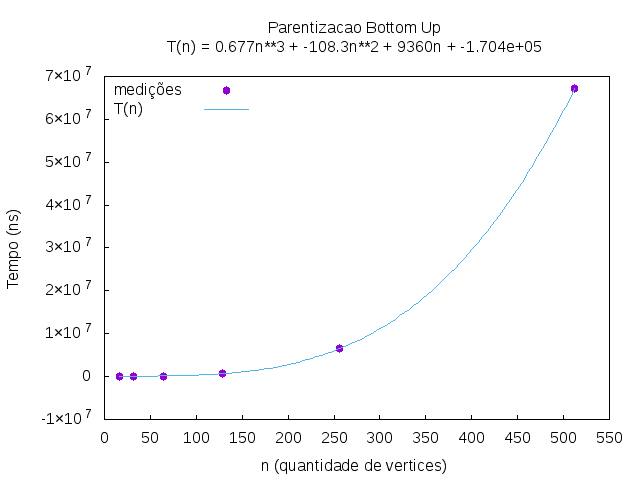
\includegraphics[width=0.7\linewidth]{graficos/Parentizacao BottomUp/Decrescente P20/ParentizacaoBottomUp.png}
  \caption{Parentização Bottom Up - Vetor Decrescente P20}
\end{figure}


\subsection{Vetor Decrescente P30}
Tabela gerada utilizando Parentização Bottom Up com vetores de tamanho n, sendo n = $(2^k)$, de k = 4..14 e inseridos Decrescente P30.
\begin{table}[H]
\centering
\caption{Parentização Bottom Up com vetor Decrescente P30}
\label{my-label}
\begin{tabular}{|l|l|}
\hline
\multicolumn{1}{|c|}{\textbf{Número de Elementos}} & \multicolumn{1}{c|}{\textbf{Tempo de execução em nanosegundos}} \\ \hline
16 & 2644 \\ \hline
32 & 14619 \\ \hline
64 & 99600 \\ \hline
128 & 771261 \\ \hline
256 & 6508011 \\ \hline
512 & 67406718 \\ \hline
\end{tabular}
\end{table}

\begin{figure}[H]
    \centering
    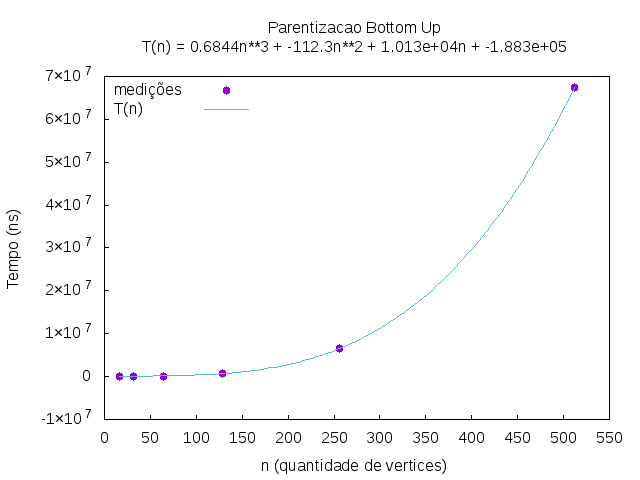
\includegraphics[width=0.7\linewidth]{graficos/Parentizacao BottomUp/Decrescente P30/ParentizacaoBottomUp.png}
  \caption{Parentização Bottom Up - Vetor Decrescente P30}
\end{figure}


\subsection{Vetor Decrescente P40}
Tabela gerada utilizando Parentização Bottom Up com vetores de tamanho n, sendo n = $(2^k)$, de k = 4..14 e inseridos Decrescente P40.
\begin{table}[H]
\centering
\caption{Parentização Bottom Up com vetor Decrescente P40}
\label{my-label}
\begin{tabular}{|l|l|}
\hline
\multicolumn{1}{|c|}{\textbf{Número de Elementos}} & \multicolumn{1}{c|}{\textbf{Tempo de execução em nanosegundos}} \\ \hline
16 & 2898 \\ \hline
32 & 15696 \\ \hline
64 & 108110 \\ \hline
128 & 760201 \\ \hline
256 & 6613108 \\ \hline
512 & 67337227 \\ \hline
\end{tabular}
\end{table}

\begin{figure}[H]
    \centering
    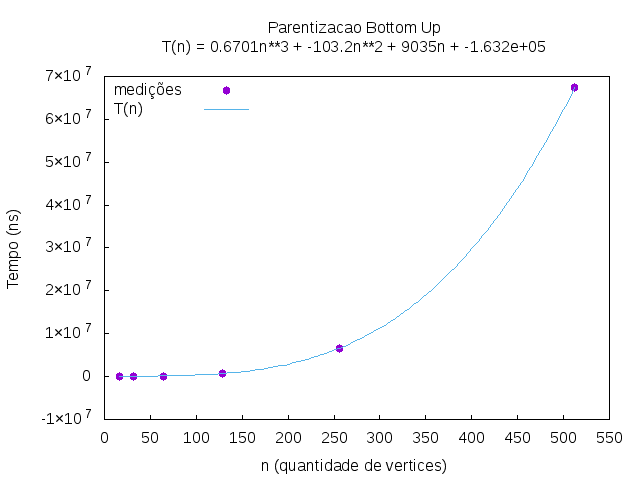
\includegraphics[width=0.7\linewidth]{graficos/Parentizacao BottomUp/Decrescente P40/ParentizacaoBottomUp.png}
  \caption{Parentização Bottom Up - Vetor Decrescente P40}
\end{figure}


\subsection{Vetor Decrescente P50}
Tabela gerada utilizando Parentização Bottom Up com vetores de tamanho n, sendo n = $(2^k)$, de k = 4..14 e inseridos Decrescente P50.
\begin{table}[H]
\centering
\caption{Parentização Bottom Up com vetor Decrescente P50}
\label{my-label}
\begin{tabular}{|l|l|}
\hline
\multicolumn{1}{|c|}{\textbf{Número de Elementos}} & \multicolumn{1}{c|}{\textbf{Tempo de execução em nanosegundos}} \\ \hline
16 & 2961 \\ \hline
32 & 16579 \\ \hline
64 & 105587 \\ \hline
128 & 771134 \\ \hline
256 & 6553364 \\ \hline
512 & 67677413 \\ \hline
\end{tabular}
\end{table}

\begin{figure}[H]
    \centering
    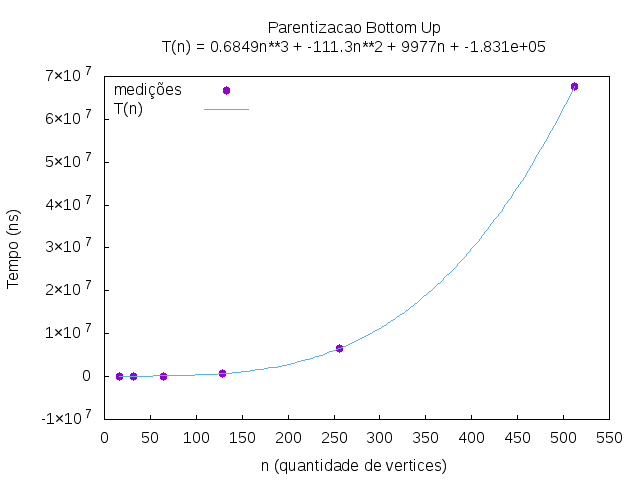
\includegraphics[width=0.7\linewidth]{graficos/Parentizacao BottomUp/Decrescente P50/ParentizacaoBottomUp.png}
  \caption{Parentização Bottom Up - Vetor Decrescente P50}
\end{figure}

\section{Parentização Recursiva}

Problema já comentado anteriormente.

\subsection{Vetor}
Tabela gerada utilizando Parentização Recursiva com vetores de tamanho n, sendo n = $(2^k)$, de k = 4, pois após isso há um estouro de memória, logo não é possível extrair um gráfico.
\begin{table}[H]
\centering
\caption{Parentização Recursiva}
\label{my-label}
\begin{tabular}{|l|l|}
\hline
\multicolumn{1}{|c|}{\textbf{Número de Elementos}} & \multicolumn{1}{c|}{\textbf{Tempo de execução em nanosegundos}} \\ \hline
16 & 103633175 \\ \hline
16 & 103633175 \\ \hline
16 & 103633175 \\ \hline
16 & 103633175 \\ \hline
16 & 103633175 \\ \hline
16 & 103633175 \\ \hline
16 & 103633175 \\ \hline
16 & 103633175 \\ \hline
16 & 103633175 \\ \hline
16 & 103633175 \\ \hline
16 & 103633175 \\ \hline
16 & 103633175 \\ \hline
16 & 103633175 \\ \hline
\end{tabular}
\end{table}

\chapter{Estatísticas de Ordem}

A iesima estatística de ordem de um conjunto com n elementos é o iesimo menor elemento desse conjunto.

\section{Min}

Mínimo é a primeira estatística de ordem, com i = 1.

\subsection{Vetor aleatorio}
Tabela gerada utilizando Min com vetores de tamanho n, sendo n = $(2^k)$, de k = 4..14 e inseridos aleatóriamente.
\begin{table}[H]
\centering
\caption{Min com vetor aleatório}
\label{my-label}
\begin{tabular}{|l|l|}
\hline
\multicolumn{1}{|c|}{\textbf{Número de Elementos}} & \multicolumn{1}{c|}{\textbf{Tempo de execução em nanosegundos}} \\ \hline
16 & 520 \\ \hline
32 & 300 \\ \hline
64 & 326 \\ \hline
128 & 358 \\ \hline
256 & 387 \\ \hline
512 & 458 \\ \hline
1024 & 1017 \\ \hline
2048 & 1227 \\ \hline
4096 & 3554 \\ \hline
8192 & 10154 \\ \hline
16384 & 6307 \\ \hline

\end{tabular}
\end{table}

\begin{figure}[H]
    \centering
    \includegraphics[width=0.7\linewidth]{graficos/Min/Aleatorio/Min.png}
  \caption{Min - Vetor Aleatório}
\end{figure}

\subsection{Vetor Crescente}
Tabela gerada utilizando Min com vetores de tamanho n, sendo n = $(2^k)$, de k = 4..14 e inseridos Crescente.
\begin{table}[H]
\centering
\caption{Min com vetor Crescente}
\label{my-label}
\begin{tabular}{|l|l|}
\hline
\multicolumn{1}{|c|}{\textbf{Número de Elementos}} & \multicolumn{1}{c|}{\textbf{Tempo de execução em nanosegundos}} \\ \hline
16 & 315 \\ \hline
32 & 426 \\ \hline
64 & 328 \\ \hline
128 & 336 \\ \hline
256 & 405 \\ \hline
512 & 496 \\ \hline
1024 & 10294 \\ \hline
2048 & 1053 \\ \hline
4096 & 1707 \\ \hline
8192 & 6034 \\ \hline
16384 & 17684 \\ \hline

\end{tabular}
\end{table}

\begin{figure}[H]
    \centering
    \includegraphics[width=0.7\linewidth]{graficos/Min/Crescente/Min.png}
  \caption{Min - Vetor Crescente}
\end{figure}


\subsection{Vetor Crescente P10}
Tabela gerada utilizando Min com vetores de tamanho n, sendo n = $(2^k)$, de k = 4..14 e inseridos Crescente P10.
\begin{table}[H]
\centering
\caption{Min com vetor Crescente P10}
\label{my-label}
\begin{tabular}{|l|l|}
\hline
\multicolumn{1}{|c|}{\textbf{Número de Elementos}} & \multicolumn{1}{c|}{\textbf{Tempo de execução em nanosegundos}} \\ \hline
16 & 393 \\ \hline
32 & 290 \\ \hline
64 & 285 \\ \hline
128 & 330 \\ \hline
256 & 371 \\ \hline
512 & 638 \\ \hline
1024 & 658 \\ \hline
2048 & 1324 \\ \hline
4096 & 2086 \\ \hline
8192 & 3680 \\ \hline
16384 & 20530 \\ \hline

\end{tabular}
\end{table}

\begin{figure}[H]
    \centering
    \includegraphics[width=0.7\linewidth]{graficos/Min/Crescente P10/Min.png}
  \caption{Min - Vetor Crescente P10}
\end{figure}


\subsection{Vetor Crescente P20}
Tabela gerada utilizando Min com vetores de tamanho n, sendo n = $(2^k)$, de k = 4..14 e inseridos Crescente P20.
\begin{table}[H]
\centering
\caption{Min com vetor Crescente P20}
\label{my-label}
\begin{tabular}{|l|l|}
\hline
\multicolumn{1}{|c|}{\textbf{Número de Elementos}} & \multicolumn{1}{c|}{\textbf{Tempo de execução em nanosegundos}} \\ \hline
16 & 805 \\ \hline
32 & 500 \\ \hline
64 & 766 \\ \hline
128 & 486 \\ \hline
256 & 427 \\ \hline
512 & 497 \\ \hline
1024 & 745 \\ \hline
2048 & 1113 \\ \hline
4096 & 3154 \\ \hline
8192 & 2949 \\ \hline
16384 & 5554 \\ \hline
\end{tabular}
\end{table}

\begin{figure}[H]
    \centering
    \includegraphics[width=0.7\linewidth]{graficos/Min/Crescente P20/Min.png}
  \caption{Min - Vetor Crescente P20}
\end{figure}

\subsection{Vetor Crescente P30}
Tabela gerada utilizando Min com vetores de tamanho n, sendo n = $(2^k)$, de k = 4..14 e inseridos Crescente P30.
\begin{table}[H]
\centering
\caption{Min com vetor Crescente P30}
\label{my-label}
\begin{tabular}{|l|l|}
\hline
\multicolumn{1}{|c|}{\textbf{Número de Elementos}} & \multicolumn{1}{c|}{\textbf{Tempo de execução em nanosegundos}} \\ \hline
16 & 304 \\ \hline
32 & 274 \\ \hline
64 & 297 \\ \hline
128 & 466 \\ \hline
256 & 390 \\ \hline
512 & 463 \\ \hline
1024 & 587 \\ \hline
2048 & 891 \\ \hline
4096 & 1554 \\ \hline
8192 & 3553 \\ \hline
16384 & 7562 \\ \hline

\end{tabular}
\end{table}

\begin{figure}[H]
    \centering
    \includegraphics[width=0.7\linewidth]{graficos/Min/Crescente P30/Min.png}
  \caption{Min - Vetor Crescente P30}
\end{figure}

\subsection{Vetor Crescente P40}
Tabela gerada utilizando Min com vetores de tamanho n, sendo n = $(2^k)$, de k = 4..14 e inseridos Crescente P40.
\begin{table}[H]
\centering
\caption{Min com vetor Crescente P40}
\label{my-label}
\begin{tabular}{|l|l|}
\hline
\multicolumn{1}{|c|}{\textbf{Número de Elementos}} & \multicolumn{1}{c|}{\textbf{Tempo de execução em nanosegundos}} \\ \hline
16 & 332 \\ \hline
32 & 330 \\ \hline
64 & 302 \\ \hline
128 & 350 \\ \hline
256 & 426 \\ \hline
512 & 466 \\ \hline
1024 & 1714 \\ \hline
2048 & 2170 \\ \hline
4096 & 4381 \\ \hline
8192 & 12724 \\ \hline
16384 & 6773 \\ \hline

\end{tabular}
\end{table}

\begin{figure}[H]
    \centering
    \includegraphics[width=0.7\linewidth]{graficos/Min/Crescente P40/Min.png}
  \caption{Min - Vetor Crescente P40}
\end{figure}

\subsection{Vetor Crescente P50}
Tabela gerada utilizando Min com vetores de tamanho n, sendo n = $(2^k)$, de k = 4..14 e inseridos Crescente P50.
\begin{table}[H]
\centering
\caption{Min com vetor Crescente P50}
\label{my-label}
\begin{tabular}{|l|l|}
\hline
\multicolumn{1}{|c|}{\textbf{Número de Elementos}} & \multicolumn{1}{c|}{\textbf{Tempo de execução em nanosegundos}} \\ \hline
16 & 312 \\ \hline
32 & 276 \\ \hline
64 & 289 \\ \hline
128 & 372 \\ \hline
256 & 365 \\ \hline
512 & 543 \\ \hline
1024 & 922 \\ \hline
2048 & 922 \\ \hline
4096 & 1538 \\ \hline
8192 & 2925 \\ \hline
16384 & 6012 \\ \hline

\end{tabular}
\end{table}

\begin{figure}[H]
    \centering
    \includegraphics[width=0.7\linewidth]{graficos/Min/Crescente P50/Min.png}
  \caption{Min - Vetor Crescente P50}
\end{figure}

\subsection{Vetor Decrescente}
Tabela gerada utilizando Min com vetores de tamanho n, sendo n = $(2^k)$, de k = 4..14 e inseridos Decrescente.
\begin{table}[H]
\centering
\caption{Min com vetor Decrescente}
\label{my-label}
\begin{tabular}{|l|l|}
\hline
\multicolumn{1}{|c|}{\textbf{Número de Elementos}} & \multicolumn{1}{c|}{\textbf{Tempo de execução em nanosegundos}} \\ \hline
16 & 305 \\ \hline
32 & 278 \\ \hline
64 & 274 \\ \hline
128 & 340 \\ \hline
256 & 368 \\ \hline
512 & 472 \\ \hline
1024 & 869 \\ \hline
2048 & 1008 \\ \hline
4096 & 2077 \\ \hline
8192 & 3849 \\ \hline
16384 & 11560 \\ \hline

\end{tabular}
\end{table}

\begin{figure}[H]
    \centering
    \includegraphics[width=0.7\linewidth]{graficos/Min/Decrescente/Min.png}
  \caption{Min - Vetor Decrescente}
\end{figure}

\subsection{Vetor Decrescente P10}
Tabela gerada utilizando Min com vetores de tamanho n, sendo n = $(2^k)$, de k = 4..14 e inseridos Decrescente P10.
\begin{table}[H]
\centering
\caption{Min com vetor Decrescente P10}
\label{my-label}
\begin{tabular}{|l|l|}
\hline
\multicolumn{1}{|c|}{\textbf{Número de Elementos}} & \multicolumn{1}{c|}{\textbf{Tempo de execução em nanosegundos}} \\ \hline
16 & 317 \\ \hline
32 & 278 \\ \hline
64 & 294 \\ \hline
128 & 345 \\ \hline
256 & 357 \\ \hline
512 & 466 \\ \hline
1024 & 661 \\ \hline
2048 & 932 \\ \hline
4096 & 1855 \\ \hline
8192 & 4558 \\ \hline
16384 & 6088 \\ \hline

\end{tabular}
\end{table}

\begin{figure}[H]
    \centering
    \includegraphics[width=0.7\linewidth]{graficos/Min/Decrescente P10/Min.png}
  \caption{Min - Vetor Decrescente P10}
\end{figure}

\subsection{Vetor Decrescente P20}
Tabela gerada utilizando Min com vetores de tamanho n, sendo n = $(2^k)$, de k = 4..14 e inseridos Decrescente P20.
\begin{table}[H]
\centering
\caption{Min com vetor Decrescente P20}
\label{my-label}
\begin{tabular}{|l|l|}
\hline
\multicolumn{1}{|c|}{\textbf{Número de Elementos}} & \multicolumn{1}{c|}{\textbf{Tempo de execução em nanosegundos}} \\ \hline
16 & 331 \\ \hline
32 & 267 \\ \hline
64 & 318 \\ \hline
128 & 361 \\ \hline
256 & 403 \\ \hline
512 & 485 \\ \hline
1024 & 713 \\ \hline
2048 & 892 \\ \hline
4096 & 1790 \\ \hline
8192 & 2965 \\ \hline
16384 & 6367 \\ \hline

\end{tabular}
\end{table}

\begin{figure}[H]
    \centering
    \includegraphics[width=0.7\linewidth]{graficos/Min/Decrescente P20/Min.png}
  \caption{Min - Vetor Decrescente P20}
\end{figure}

\subsection{Vetor Decrescente P30}
Tabela gerada utilizando Min com vetores de tamanho n, sendo n = $(2^k)$, de k = 4..14 e inseridos Decrescente P30.
\begin{table}[H]
\centering
\caption{Min com vetor Decrescente P30}
\label{my-label}
\begin{tabular}{|l|l|}
\hline
\multicolumn{1}{|c|}{\textbf{Número de Elementos}} & \multicolumn{1}{c|}{\textbf{Tempo de execução em nanosegundos}} \\ \hline
16 & 335 \\ \hline
32 & 300 \\ \hline
64 & 370 \\ \hline
128 & 364 \\ \hline
256 & 433 \\ \hline
512 & 503 \\ \hline
1024 & 678 \\ \hline
2048 & 1236 \\ \hline
4096 & 2175 \\ \hline
8192 & 9572 \\ \hline
16384 & 13543 \\ \hline

\end{tabular}
\end{table}

\begin{figure}[H]
    \centering
    \includegraphics[width=0.7\linewidth]{graficos/Min/Decrescente P30/Min.png}
  \caption{Min - Vetor Decrescente P30}
\end{figure}

\subsection{Vetor Decrescente P40}
Tabela gerada utilizando Min com vetores de tamanho n, sendo n = $(2^k)$, de k = 4..14 e inseridos Decrescente P40.
\begin{table}[H]
\centering
\caption{Min com vetor Decrescente P40}
\label{my-label}
\begin{tabular}{|l|l|}
\hline
\multicolumn{1}{|c|}{\textbf{Número de Elementos}} & \multicolumn{1}{c|}{\textbf{Tempo de execução em nanosegundos}} \\ \hline
16 & 323 \\ \hline
32 & 279 \\ \hline
64 & 358 \\ \hline
128 & 342 \\ \hline
256 & 363 \\ \hline
512 & 469 \\ \hline
1024 & 659 \\ \hline
2048 & 899 \\ \hline
4096 & 1831 \\ \hline
8192 & 2947 \\ \hline
16384 & 5499 \\ \hline

\end{tabular}
\end{table}

\begin{figure}[H]
    \centering
    \includegraphics[width=0.7\linewidth]{graficos/Min/Decrescente P40/Min.png}
  \caption{Min - Vetor Decrescente P40}
\end{figure}

\subsection{Vetor Decrescente P50}
Tabela gerada utilizando Min com vetores de tamanho n, sendo n = $(2^k)$, de k = 4..14 e inseridos Decrescente P50.
\begin{table}[H]
\centering
\caption{Min com vetor Decrescente P50}
\label{my-label}
\begin{tabular}{|l|l|}
\hline
\multicolumn{1}{|c|}{\textbf{Número de Elementos}} & \multicolumn{1}{c|}{\textbf{Tempo de execução em nanosegundos}} \\ \hline
16 & 341 \\ \hline
32 & 300 \\ \hline
64 & 320 \\ \hline
128 & 361 \\ \hline
256 & 422 \\ \hline
512 & 460 \\ \hline
1024 & 637 \\ \hline
2048 & 1070 \\ \hline
4096 & 1853 \\ \hline
8192 & 2951 \\ \hline
16384 & 7247 \\ \hline
\end{tabular}
\end{table}

\begin{figure}[H]
    \centering
    \includegraphics[width=0.7\linewidth]{graficos/Min/Decrescente P50/Min.png}
  \caption{Min - Vetor Decrescente P50}
\end{figure}




\section{MinMax}

Mínimo é a primeira estatística de ordem, com i = 1.
Máximo é a n ésima estatística de ordem, com i = n.

\subsection{Vetor aleatorio}
Tabela gerada utilizando MinMax com vetores de tamanho n, sendo n = $(2^k)$, de k = 4..14 e inseridos aleatóriamente.
\begin{table}[H]
\centering
\caption{MinMax com vetor aleatório}
\label{my-label}
\begin{tabular}{|l|l|}
\hline
\multicolumn{1}{|c|}{\textbf{Número de Elementos}} & \multicolumn{1}{c|}{\textbf{Tempo de execução em nanosegundos}} \\ \hline
16 & 834 \\ \hline
32 & 444 \\ \hline
64 & 460 \\ \hline
128 & 455 \\ \hline
256 & 545 \\ \hline
512 & 685 \\ \hline
1024 & 974 \\ \hline
2048 & 1322 \\ \hline
4096 & 2133 \\ \hline
8192 & 3744 \\ \hline
16384 & 8385 \\ \hline
\end{tabular}
\end{table}

\begin{figure}[H]
    \centering
    \includegraphics[width=0.7\linewidth]{graficos/Min Max/Aleatorio/MinMax.png}
  \caption{MinMax - Vetor Aleatório}
\end{figure}

\subsection{Vetor Crescente}
Tabela gerada utilizando MinMax com vetores de tamanho n, sendo n = $(2^k)$, de k = 4..14 e inseridos Crescente.
\begin{table}[H]
\centering
\caption{MinMax com vetor Crescente}
\label{my-label}
\begin{tabular}{|l|l|}
\hline
\multicolumn{1}{|c|}{\textbf{Número de Elementos}} & \multicolumn{1}{c|}{\textbf{Tempo de execução em nanosegundos}} \\ \hline
16 & 554 \\ \hline
32 & 442 \\ \hline
64 & 460 \\ \hline
128 & 457 \\ \hline
256 & 508 \\ \hline
512 & 672 \\ \hline
1024 & 1444 \\ \hline
2048 & 1928 \\ \hline
4096 & 10075 \\ \hline
8192 & 8232 \\ \hline
16384 & 8076 \\ \hline
\end{tabular}
\end{table}

\begin{figure}[H]
    \centering
    \includegraphics[width=0.7\linewidth]{graficos/Min Max/Crescente/MinMax.png}
  \caption{MinMax - Vetor Crescente}
\end{figure}

\subsection{Vetor Crescente P10}
Tabela gerada utilizando MinMax com vetores de tamanho n, sendo n = $(2^k)$, de k = 4..14 e inseridos Crescente P10.
\begin{table}[H]
\centering
\caption{MinMax com vetor Crescente P10}
\label{my-label}
\begin{tabular}{|l|l|}
\hline
\multicolumn{1}{|c|}{\textbf{Número de Elementos}} & \multicolumn{1}{c|}{\textbf{Tempo de execução em nanosegundos}} \\ \hline
16 & 510 \\ \hline
32 & 472 \\ \hline
64 & 513 \\ \hline
128 & 434 \\ \hline
256 & 551 \\ \hline
512 & 712 \\ \hline
1024 & 881 \\ \hline
2048 & 1535 \\ \hline
4096 & 2929 \\ \hline
8192 & 8249 \\ \hline
16384 & 22516 \\ \hline
\end{tabular}
\end{table}

\begin{figure}[H]
    \centering
    \includegraphics[width=0.7\linewidth]{graficos/Min Max/Crescente P10/MinMax.png}
  \caption{MinMax - Vetor Crescente P10}
\end{figure}

\subsection{Vetor Crescente P20}
Tabela gerada utilizando MinMax com vetores de tamanho n, sendo n = $(2^k)$, de k = 4..14 e inseridos Crescente P20.
\begin{table}[H]
\centering
\caption{MinMax com vetor Crescente P20}
\label{my-label}
\begin{tabular}{|l|l|}
\hline
\multicolumn{1}{|c|}{\textbf{Número de Elementos}} & \multicolumn{1}{c|}{\textbf{Tempo de execução em nanosegundos}} \\ \hline
16 & 454 \\ \hline
32 & 465 \\ \hline
64 & 461 \\ \hline
128 & 472 \\ \hline
256 & 525 \\ \hline
512 & 650 \\ \hline
1024 & 1049 \\ \hline
2048 & 1335 \\ \hline
4096 & 2398 \\ \hline
8192 & 3837 \\ \hline
16384 & 7720 \\ \hline
\end{tabular}
\end{table}

\begin{figure}[H]
    \centering
    \includegraphics[width=0.7\linewidth]{graficos/Min Max/Crescente P20/MinMax.png}
  \caption{MinMax - Vetor Crescente P20}
\end{figure}

\subsection{Vetor Crescente P30}
Tabela gerada utilizando MinMax com vetores de tamanho n, sendo n = $(2^k)$, de k = 4..14 e inseridos Crescente P30.
\begin{table}[H]
\centering
\caption{MinMax com vetor Crescente P30}
\label{my-label}
\begin{tabular}{|l|l|}
\hline
\multicolumn{1}{|c|}{\textbf{Número de Elementos}} & \multicolumn{1}{c|}{\textbf{Tempo de execução em nanosegundos}} \\ \hline
16 & 445 \\ \hline
32 & 533 \\ \hline
64 & 484 \\ \hline
128 & 423 \\ \hline
256 & 544 \\ \hline
512 & 676 \\ \hline
1024 & 847 \\ \hline
2048 & 1323 \\ \hline
4096 & 2201 \\ \hline
8192 & 3786 \\ \hline
16384 & 10934 \\ \hline
\end{tabular}
\end{table}

\begin{figure}[H]
    \centering
    \includegraphics[width=0.7\linewidth]{graficos/Min Max/Crescente P30/MinMax.png}
  \caption{MinMax - Vetor Crescente P30}
\end{figure}

\subsection{Vetor Crescente P40}
Tabela gerada utilizando MinMax com vetores de tamanho n, sendo n = $(2^k)$, de k = 4..14 e inseridos Crescente P40.
\begin{table}[H]
\centering
\caption{MinMax com vetor Crescente P40}
\label{my-label}
\begin{tabular}{|l|l|}
\hline
\multicolumn{1}{|c|}{\textbf{Número de Elementos}} & \multicolumn{1}{c|}{\textbf{Tempo de execução em nanosegundos}} \\ \hline
16 & 1292 \\ \hline
32 & 483 \\ \hline
64 & 573 \\ \hline
128 & 807 \\ \hline
256 & 562 \\ \hline
512 & 1705 \\ \hline
1024 & 2362 \\ \hline
2048 & 3904 \\ \hline
4096 & 5994 \\ \hline
8192 & 4047 \\ \hline
16384 & 7145 \\ \hline
\end{tabular}
\end{table}

\begin{figure}[H]
    \centering
    \includegraphics[width=0.7\linewidth]{graficos/Min Max/Crescente P40/MinMax.png}
  \caption{MinMax - Vetor Crescente P40}
\end{figure}

\subsection{Vetor Crescente P50}
Tabela gerada utilizando MinMax com vetores de tamanho n, sendo n = $(2^k)$, de k = 4..14 e inseridos Crescente P50.
\begin{table}[H]
\centering
\caption{MinMax com vetor Crescente P50}
\label{my-label}
\begin{tabular}{|l|l|}
\hline
\multicolumn{1}{|c|}{\textbf{Número de Elementos}} & \multicolumn{1}{c|}{\textbf{Tempo de execução em nanosegundos}} \\ \hline
16 & 460 \\ \hline
32 & 463 \\ \hline
64 & 464 \\ \hline
128 & 496 \\ \hline
256 & 948 \\ \hline
512 & 688 \\ \hline
1024 & 854 \\ \hline
2048 & 1308 \\ \hline
4096 & 2643 \\ \hline
8192 & 5058 \\ \hline
16384 & 7017 \\ \hline
\end{tabular}
\end{table}

\begin{figure}[H]
    \centering
    \includegraphics[width=0.7\linewidth]{graficos/Min Max/Crescente P50/MinMax.png}
  \caption{MinMax - Vetor Crescente P50}
\end{figure}

\subsection{Vetor Decrescente}
Tabela gerada utilizando MinMax com vetores de tamanho n, sendo n = $(2^k)$, de k = 4..14 e inseridos Decrescente.
\begin{table}[H]
\centering
\caption{MinMax com vetor Decrescente}
\label{my-label}
\begin{tabular}{|l|l|}
\hline
\multicolumn{1}{|c|}{\textbf{Número de Elementos}} & \multicolumn{1}{c|}{\textbf{Tempo de execução em nanosegundos}} \\ \hline
16 & 440 \\ \hline
32 & 394 \\ \hline
64 & 488 \\ \hline
128 & 444 \\ \hline
256 & 511 \\ \hline
512 & 659 \\ \hline
1024 & 1000 \\ \hline
2048 & 1525 \\ \hline
4096 & 2986 \\ \hline
8192 & 6276 \\ \hline
16384 & 15652 \\ \hline
\end{tabular}
\end{table}

\begin{figure}[H]
    \centering
    \includegraphics[width=0.7\linewidth]{graficos/Min Max/Decrescente/MinMax.png}
  \caption{MinMax - Vetor Decrescente}
\end{figure}

\subsection{Vetor Decrescente P10}
Tabela gerada utilizando MinMax com vetores de tamanho n, sendo n = $(2^k)$, de k = 4..14 e inseridos Decrescente P10.
\begin{table}[H]
\centering
\caption{MinMax com vetor Decrescente P10}
\label{my-label}
\begin{tabular}{|l|l|}
\hline
\multicolumn{1}{|c|}{\textbf{Número de Elementos}} & \multicolumn{1}{c|}{\textbf{Tempo de execução em nanosegundos}} \\ \hline
16 & 448 \\ \hline
32 & 428 \\ \hline
64 & 445 \\ \hline
128 & 599 \\ \hline
256 & 488 \\ \hline
512 & 656 \\ \hline
1024 & 876 \\ \hline
2048 & 1299 \\ \hline
4096 & 2130 \\ \hline
8192 & 3922 \\ \hline
16384 & 8388 \\ \hline
\end{tabular}
\end{table}

\begin{figure}[H]
    \centering
    \includegraphics[width=0.7\linewidth]{graficos/Min Max/Decrescente P10/MinMax.png}
  \caption{MinMax - Vetor Decrescente P10}
\end{figure}

\subsection{Vetor Decrescente P20}
Tabela gerada utilizando MinMax com vetores de tamanho n, sendo n = $(2^k)$, de k = 4..14 e inseridos Decrescente P20.
\begin{table}[H]
\centering
\caption{MinMax com vetor Decrescente P20}
\label{my-label}
\begin{tabular}{|l|l|}
\hline
\multicolumn{1}{|c|}{\textbf{Número de Elementos}} & \multicolumn{1}{c|}{\textbf{Tempo de execução em nanosegundos}} \\ \hline
16 & 416 \\ \hline
32 & 477 \\ \hline
64 & 461 \\ \hline
128 & 464 \\ \hline
256 & 576 \\ \hline
512 & 749 \\ \hline
1024 & 864 \\ \hline
2048 & 1238 \\ \hline
4096 & 2019 \\ \hline
8192 & 3970 \\ \hline
16384 & 9291 \\ \hline
\end{tabular}
\end{table}

\begin{figure}[H]
    \centering
    \includegraphics[width=0.7\linewidth]{graficos/Min Max/Decrescente P20/MinMax.png}
  \caption{MinMax - Vetor Decrescente P20}
\end{figure}

\subsection{Vetor Decrescente P30}
Tabela gerada utilizando MinMax com vetores de tamanho n, sendo n = $(2^k)$, de k = 4..14 e inseridos Decrescente P30.
\begin{table}[H]
\centering
\caption{MinMax com vetor Decrescente P30}
\label{my-label}
\begin{tabular}{|l|l|}
\hline
\multicolumn{1}{|c|}{\textbf{Número de Elementos}} & \multicolumn{1}{c|}{\textbf{Tempo de execução em nanosegundos}} \\ \hline
16 & 481 \\ \hline
32 & 429 \\ \hline
64 & 480 \\ \hline
128 & 480 \\ \hline
256 & 534 \\ \hline
512 & 723 \\ \hline
1024 & 1062 \\ \hline
2048 & 2273 \\ \hline
4096 & 6007 \\ \hline
8192 & 13578 \\ \hline
16384 & 7634 \\ \hline
\end{tabular}
\end{table}

\begin{figure}[H]
    \centering
    \includegraphics[width=0.7\linewidth]{graficos/Min Max/Decrescente P30/MinMax.png}
  \caption{MinMax - Vetor Decrescente P30}
\end{figure}

\subsection{Vetor Decrescente P40}
Tabela gerada utilizando MinMax com vetores de tamanho n, sendo n = $(2^k)$, de k = 4..14 e inseridos Decrescente P40.
\begin{table}[H]
\centering
\caption{MinMax com vetor Decrescente P40}
\label{my-label}
\begin{tabular}{|l|l|}
\hline
\multicolumn{1}{|c|}{\textbf{Número de Elementos}} & \multicolumn{1}{c|}{\textbf{Tempo de execução em nanosegundos}} \\ \hline
16 & 484 \\ \hline
32 & 472 \\ \hline
64 & 440 \\ \hline
128 & 462 \\ \hline
256 & 486 \\ \hline
512 & 664 \\ \hline
1024 & 1036 \\ \hline
2048 & 1507 \\ \hline
4096 & 2219 \\ \hline
8192 & 3887 \\ \hline
16384 & 7530 \\ \hline
\end{tabular}
\end{table}

\begin{figure}[H]
    \centering
    \includegraphics[width=0.7\linewidth]{graficos/Min Max/Decrescente P40/MinMax.png}
  \caption{MinMax - Vetor Decrescente P40}
\end{figure}

\subsection{Vetor Decrescente P50}
Tabela gerada utilizando MinMax com vetores de tamanho n, sendo n = $(2^k)$, de k = 4..14 e inseridos Decrescente P50.
\begin{table}[H]
\centering
\caption{MinMax com vetor Decrescente P50}
\label{my-label}
\begin{tabular}{|l|l|}
\hline
\multicolumn{1}{|c|}{\textbf{Número de Elementos}} & \multicolumn{1}{c|}{\textbf{Tempo de execução em nanosegundos}} \\ \hline
16 & 415 \\ \hline
32 & 494 \\ \hline
64 & 408 \\ \hline
128 & 453 \\ \hline
256 & 507 \\ \hline
512 & 672 \\ \hline
1024 & 806 \\ \hline
2048 & 1413 \\ \hline
4096 & 2813 \\ \hline
8192 & 4791 \\ \hline
16384 & 25421 \\ \hline
\end{tabular}
\end{table}

\begin{figure}[H]
    \centering
    \includegraphics[width=0.7\linewidth]{graficos/Min Max/Decrescente P50/MinMax.png}
  \caption{MinMax - Vetor Decrescente P50}
\end{figure}

\section{Seleciona Aleatorizado}
Algoritmo inspirado no Quicksort que resolve o problema da seleção.
\subsection{Vetor aleatorio}
Tabela gerada utilizando Seleciona Aleatorizado com vetores de tamanho n, sendo n = $(2^k)$, de k = 4..14 e inseridos aleatóriamente.
\begin{table}[H]
\centering
\caption{Seleciona Aleatorizado com vetor aleatório}
\label{my-label}
\begin{tabular}{|l|l|}
\hline
\multicolumn{1}{|c|}{\textbf{Número de Elementos}} & \multicolumn{1}{c|}{\textbf{Tempo de execução em nanosegundos}} \\ \hline
16 & 631 \\ \hline
32 & 664 \\ \hline
64 & 732 \\ \hline
128 & 764 \\ \hline
256 & 968 \\ \hline
512 & 1068 \\ \hline
1024 & 1332 \\ \hline
2048 & 2044 \\ \hline
4096 & 3555 \\ \hline
8192 & 6672 \\ \hline
16384 & 12553 \\ \hline

\end{tabular}
\end{table}

\begin{figure}[H]
    \centering
    \includegraphics[width=0.7\linewidth]{graficos/SelecionaAleatorizado/SeletorRecursivoAtividades.png}
  \caption{Seleciona Aleatorizado - Vetor Aleatório}
\end{figure}

%para ajuda
%\lstinputlisting[label={arq:prog1.c}, language=C, caption={Módulo Mínimo C}]{codigos/MiniC/prog1.c}
%\lstinputlisting[label={arq:prog4.c}, language=C, caption={Atribuição de uma soma de inteiros a uma variável C}]{codigos/MiniC/prog4.c}
%\begin{terminal}
%> sudo apt-get install llvm
%> sudo apt-get install clang
%\end{terminal}

\chapter{Referências}
\href{https://en.wikipedia.org/wiki/Busca_em_largura}{Busca em Largura}\\
\href{https://en.wikipedia.org/wiki/Busca_em_profundidade}{Busca em Profundidade}\\
\href{https://pt.wikipedia.org/wiki/Codificação_de_Huffman}{Huffman}\\
\href{http://www.cplusplus.com/reference/algorithm/min_element}{Min}\\
\href{http://en.cppreference.com/w/cpp/algorithm/minmax_element}{Min Max}\\
\href{https://pt.wikipedia.org/wiki/Problema_da_mochila}{Mochila Fracionada}\\
\href{https://pt.wikipedia.org/wiki/Ordenação_topológica}{Ordenação Tolológica}\\
\href{https://groups.google.com/forum/#!topic/gbc052/}{Slides Professor}\\
Introduction to algorithms 3rd Edition,Cormen, Thomas H,2009
  
\end{document} 
